\documentclass[twoside,a4paper,11pt]{book}
\usepackage[english]{babel}

\usepackage[utf8]{inputenc}
\usepackage[T1]{fontenc}
\usepackage{url}
\usepackage[pdftex]{graphicx}
\usepackage{a4wide}
\usepackage{geometry}
\usepackage[backend=bibtex]{biblatex}
\usepackage{hyperref}
\usepackage{subfiles}
\usepackage[normalsize]{subfigure}
\usepackage{color}
\usepackage{amsmath}
\usepackage{amsfonts}
\usepackage[normalem]{ulem}
\usepackage{float}
\usepackage{enumitem}
\usepackage{mathtools}
\usepackage{listings}
\usepackage{textcomp}
\usepackage{tikz}
\usepackage{verbatim}
\usepackage{forest}
\usepackage{fontawesome}

\setcounter{tocdepth}{4}
\setcounter{secnumdepth}{4}

% For using margin notes instead of marginpar
\usepackage{marginnote}
% Margin notes smaller that default
\renewcommand*{\marginfont}{\footnotesize}
\newcommand{\myparagraph}[1]{\paragraph{#1}\mbox{}\\}

\addto\captionsenglish{\renewcommand{\chaptername}{Capítulo}}
\addto\captionsenglish{\renewcommand{\contentsname}{Índice}}
\addto\captionsenglish{\renewcommand{\listfigurename}{Lista de figuras}}

\lstset{
    backgroundcolor=\color[rgb]{0.95, 0.95, 0.95},
    tabsize=2,
    rulecolor=,
    basicstyle=\scriptsize,
    upquote=true,
    aboveskip={1.5\baselineskip},
    columns=fixed,
    showstringspaces=false,
    extendedchars=true,
    breaklines=true,
    prebreak = \raisebox{0ex}[0ex][0ex]{\ensuremath{\hookleftarrow}},
    frame=single,
    showtabs=false,
    showspaces=false,
    showstringspaces=false,
    identifierstyle=\ttfamily,
    keywordstyle=\color[rgb]{1.0,0,0},
    keywordstyle=[1]\color[rgb]{0,0,0.75},
    keywordstyle=[2]\color[rgb]{0.5,0.0,0.0},
    keywordstyle=[3]\color[rgb]{0.127,0.427,0.514},
    keywordstyle=[4]\color[rgb]{0.4,0.4,0.4},
    commentstyle=\color[rgb]{0.133,0.545,0.133},
    stringstyle=\color[rgb]{0.639,0.082,0.082},
}

\lstdefinestyle{java} {
    language=Java,
    morekeywords={record, var}
}

\newcommand{\basictree}[1]{\begin{forest}
    for tree={
        font=\ttfamily,
        grow'=0,
        child anchor=west,
        parent anchor=south,
        anchor=west,
        calign=first,
        edge path={
            \noexpand\path [draw, \forestoption{edge}]
            (!u.south west) +(7.5pt,0) |- node[fill,inner sep=1.25pt] {} (.child anchor)\forestoption{edge label};
        },
        before typesetting nodes={
            if n=1
                {insert before={[,phantom]}}
                {}
        },
        fit=band,
        before computing xy={l=15pt},
    }
    #1
\end{forest}}

\DeclareGraphicsExtensions{.png, .jpg, .pdf, .eps, .tiff}
\DeclareGraphicsRule{.eps}{pdf}{.pdf}{pdf}
\pdfcompresslevel=9
\geometry{a4paper, left=2.6cm, right=2.2cm, top=3.0cm, bottom=3.0cm}
\linespread{1.2}
\setlength{\parskip}{1ex plus 0.5ex minus 0.2ex}

\bibliography{main}

\begin{document}
    \thispagestyle{empty}


\includegraphics{images/URJC_logo}
\vspace{2cm}

\begin{center}
	\large{\textbf{ESCUELA TÉCNICA SUPERIOR DE INGENIERÍA INFORMÁTICA}}
	\vspace{5mm}

 	{\Large {Grado en Ingeniería de Computadores}}
    \\
  	\vspace{34mm}
	{\large {\bf TRABAJO FIN DE GRADO}}
  	\vspace{10mm}
    \\
  	{\Large {{\Huge {
  		JAMS: entorno moderno de desarrollo para MIPS32 con un enfoque educativo
	}} \\[1cm] }}
  	\vspace{2cm}
	{\large {
        \textbf{Autor}: Gael Rial Costas\\
        \textbf{Tutores}:\\
        Luis Rincón Córcoles\\
        Óscar David Robles Sánchez\\
  	}}
	\vspace{10mm}
  	{\large {Curso académico 2021/2022}}
  	\vspace{1cm}
\end{center}

    \clearpage
    \thispagestyle{empty}
    \vspace{5cm}
    \frontmatter
    \chapter{Resumen} \label{ch:resumen}

Este Trabajo \delODR{de} Fin de Grado contempla el diseño y desarrollo de \textit{JAMS},
un entorno de desarrollo integrado moderno, ligero y altamente modificable
para proyectos en lenguaje ensamblador.
El entorno de desarrollo incorpora por defecto un editor, ensamblador y simulador
para la arquitectura \textit{MIPS32}, con un enfoque educativo.
Para ello, la aplicación presenta varias herramientas que permiten
visualizar el estado del proyecto desde diferentes puntos de vista.\\
Con esto, se pretende contribuir \delODR{en}\newODR{a} una enseñanza de mejor calidad para
los alumnos que cursan alguna asignatura relacionada con arquitectura\delODR{s}\newODR{ de computadores},
procesadores o lenguajes de programación de bajo nivel.

    \chapter{Abstract} \label{ch:abstract}

This Bachelor's Thesis to obtain the Degree of Coputing Engineering contemplates the design and development of \textit{JAMS},
a modern, lightweight and highly modifiable integrated
development environment for assembly language projects.
The development environment incorporates by default an editor,
assembler and simulator for the MIPS32 architecture, with an educational approach.
For this purpose, the application presents several tools that allow visualizing
the project status from different points of view.
With this, it is intended to contribute to a better quality
teaching for students taking a subject related to computer architecture,
processors or low-level programming languages.

    \tableofcontents
    \listoffigures
    \mainmatter
    \chapter{Descripción del problema} \label{ch:descripcion-del-problema}


\section{Definición de conceptos}\label{sec:definicion-de-conceptos}

\subsection{La arquitectura \textit{MIPS}}\label{subsec:la-arquitectura-mips}

Se conoce con el nombre de \textbf{procesadores \textit{MIPS}}
\footnote{Creado por \emph{MIPS Computer Systems}, en la actualidad \emph{MIPS Technologies}}
a una familia de microprocesadores que implementan
la arquitectura \textit{RISC} del mismo nombre.
Aunque esta arquitectura no ha tenido un gran éxito en los computadores personales, sí ha gozado de fama en
sistemas empotrados, enrutadores, videoconsolas como la \textit{Nintendo 64} o la \textit{PlayStation 2},
y en máquinas utilizadas en diferentes aplicaciones, como las estaciones \textit{SGI IRIS 4D}
creadas por \textit{Silicon Graphics, Inc.} y empleadas en la industria cinematográfica para
la creación de animaciones y la generación de efectos especiales.

Su simple diseño y baja curva de aprendizaje hace a esta arquitectura ideal para introducir a los alumnos
a los lenguajes ensambladores.

\subsection{\textit{IDEs}: entornos de desarrollo integrados}\label{subsec:ides-entornos-de-desarrollo-integrados}

Un \textbf{entorno de desarrollo integrado} (\textit{IDE, Integrated Development Environment}) es una aplicación
informática con diversas herramientas empleadas en el desarrollo, construcción y depuración de \textit{software}.
Un \textit{IDE} suele estar desarrollado con dos objetivos clave en mente: maximizar la productividad del
desarrollador y evitar que este tenga que utilizar herramientas externas en su trabajo.

Existe una gran variedad de entornos de desarrollo en el mercado.
Estos se pueden clasificar de diferentes maneras.

\textbf{Según su propósito:}
\begin{itemize}
    \item \textbf{Entornos de desarrollo específicos:} son entornos pensados para el desarrollo en una
    tecnología concreta.
    Algunos ejemplos son \textit{NetBeans}, \textit{CLion} o \textit{Android Studio}.
    \item \textbf{Entornos de desarrollo generales:} son entornos que no se centran en una tecnología en concreto.
    Algunos ejemplos son \textit{IntelliJ IDEA}\cite{INTELLIJIDEA},
    \textit{Eclipse}\cite{ECLIPSE} o \textit{Microsoft Visual Studio}\cite{VISUALSTUDIO}
\end{itemize}

\textbf{Según su complejidad:}
\begin{itemize}
    \item \textbf{Entornos de desarrollo complejos:} son aplicaciones pesadas con una gran cantidad de
    características y funcionalidades.
    Algunos ejemplos son \textit{IntelliJ IDEA},
    \textit{Microsoft Visual Studio} o \textit{Eclipse}.
    \item \textbf{Entornos de desarrollo ligeros:} son aplicaciones que ocupan muy poco espacio, donde
    las características más avanzadas suelen ser componentes descargables.
    Algunos ejemplos son \textit{Visual Studio Code}\cite{VISUALSTUDIOCODE},
    \textit{Atom}\cite{ATOM} o \textit{Notepad++}\cite{NOTEPADPP}.
\end{itemize}

\subsection{Simuladores y emuladores}
\label{subsec:simuladores-y-emuladores}

Tanto un simulador como un emulador puede definirse como un
programa de computador que imita el funcionamiento de uno o varios
componentes \textit{hardware}.
Un emulador o simulador imita a una arquitectura, permitiendo
ejecutar aplicaciones ajenas a la arquitectura del computador anfitrión.

Es importante diferenciar los conceptos de \textbf{simulación}
y \textbf{emulación} a la hora de crear un programa que ejecute
código de arquitecturas externas.
La diferencia entre los simuladores y emuladores se manifiesta
en la manera en la que se implementan.

Un emulador tiene como objetivo \textbf{imitar el resultado}
que la arquitectura imitada produce al ejecutar un programa, sin tener
en cuenta el proceso interno que produce dicho resultado.
Los emuladores tienden a ser rápidos, intentando producir el resultado
de la manera más rápida y fiel posible.

Los simuladores tienen como objetivo \textbf{imitar el proceso}
que produce el resultado, simulando todos los componentes de la arquitectura.
Los simuladores tienden a ser más lentos que los emuladores, pero son más
adecuados para desarrollar y depurar aplicaciones para la arquitectura
imitada aunque no se disponga físicamente del \textit{hardware}.


\section{Descripción del problema}\label{sec:descripcion-del-problema}

Como se verá más adelante, los simuladores de la arquitectura \textit{MIPS} tuvieron
un auge importante a principios del milenio, con herramientas como \textit{MARS}\cite{MARS}
o \textit{EduMIPS64}\cite{EDUMIPS64}.
Estas herramientas estaban centradas principalmente en el \textbf{ámbito educativo}, proporcionando
interfaces sencillas y pocas herramientas.
Con el paso de los años, estas herramientas han quedado obsoletas, impidiendo desarrollar aplicaciones
en ensamblador \textit{MIPS32} de una manera cómoda.

Los principales problemas que presentan estas aplicaciones son los siguientes:
\begin{itemize}
    \item \textbf{Falta de herramientas}: los entornos de desarrollo \textit{MIPS} sufren de una
    carencia grave de herramientas importantes.
    Este problema afecta principalmente a programas como \textit{EduMIPS64}, donde no existe un editor de texto y
    el ensamblador es una aplicación separada que require la línea de comandos para funcionar.
    \item \textbf{Falta de estructura de proyecto}: a excepción de MARS, que lo hace de forma muy rudimentaria,
    ninguna aplicación actual presenta una estructura
    de proyecto, indispensable para el desarrollo de aplicaciones medianas y grandes.
    \item \textbf{Falta de personalización}: al ser aplicaciones muy sencillas, ninguna permite
    personalizar la apariencia de la interfaz.
    \item \textbf{Obsolescencia}: las aplicaciones están desarrolladas con tecnologías antiguas,
    con interfaces similares a las de los programas de principio de siglo.
    \item \textbf{Falta de capacidad de expansión}: el problema más grave que presentan estas aplicaciones
    es la poca capacidad de expansión de sus características, impidiendo que otros desarrolladores
    añadan nuevas funcionalidades de manera sencilla.
    \textit{MARS} es de los pocos entornos de desarrollo que permite expandir
    sus características mediante componentes,
    aunque su funcionamiento es muy rudimentario: el usuario debe modificar el archivo ejecutable
    para añadir nuevas herramientas.
\end{itemize}


\section{Objetivos}\label{sec:objetivos}

El objetivo principal de este proyecto es el desarrollo de \textbf{\textit{JAMS}
(\textit{Just Another MIPS Simulator})}, un \textbf{entorno de desarrollo integrado ligero, expandible y moderno}
centrado en los lenguajes ensambladores y, más concretamente,
en el lenguaje ensamblador de la arquitectura \textit{MIPS}.
Específicamente, en este apartado se detallarán diferentes objetivos.

\subsection{Investigar sobre las tecnologías más adecuadas para el desarrollo}
\label{subsec:investigar-sobre-las-tecnologias-mas-adecuados-para-el-desarrollo}

La tecnología usada en un proyecto tiene mucho peso en el resultado final.
Por ello, se debe buscar un conjunto de tecnologías que permitan crear una aplicación
moderna, multiplataforma y expandible.

Este objetivo puede separarse en dos pasos:
\begin{itemize}
    \item Elegir un lenguaje de programación con capacidad para crear aplicaciones modernas,
    que permita cargar código externo a voluntad y que tenga un buen rendimiento
    tanto en la ejecución como en el desarrollo.
    \item Seleccionar un \textit{framework} de desarrollo de aplicaciones de escritorio
    que permita desarrollar aplicaciones modernas y de gran
    calidad, dentro de las posibilidades del lenguaje de
    programación seleccionado.
\end{itemize}

\subsection{Crear un entorno base y un \textit{framework} que permita implementar diferentes herramientas}
\label{subsec:crear-un-entorno-base-y-un-framework-que-permita-implementar-diferentes-herramientas}

\textit{JAMS} pretende ser un entorno de desarrollo completamente modificable.
La mejor manera para conseguirlo es crear una base genérica
que se pueda ajustar posteriormente al desarrollo de una tecnología en concreto.

Esta base debe poder personalizar cualquier aspecto de la aplicación,
desde modificar simples mensajes y parámetros hasta añadir nuevas herramientas.
Estas modificaciones pueden venir de diferentes fuentes como
los paquetes de idiomas, los paquetes de temas y los complementos.

Por último, \textit{JAMS} debe permitir al usuario configurar los parámetros
de la aplicación de manera sencilla, proporcionando una interfaz de configuración
cómoda de utilizar.

Para conseguir este resultado, se proponen los siguientes subobjetivos:
\begin{itemize}
    \item Desarrollar una aplicación base en conjunto con una \textit{API} que pueda
    utilizarse por las diferentes herramientas para tecnologías concretas.
    \item Desarrollar e investigar diferentes formatos que permitan guardar
    y modificar los diferentes elementos estáticos de la aplicación, como
    los idiomas, los temas y la configuración, por ejemplo.
\end{itemize}

Este objetivo está relacionado con los
objetivos del Trabajo Fin de Grado del Grado en
Diseño y Desarrollo de Videojuegos de
la misma autoría que este Trabajo Fin de Grado:
desarrollar un \textbf{sistema de carga
dinámica de componentes} que permita al usuario activar y desactivar
componentes a voluntad sin tener que reiniciar la aplicación, así como
desarrollar tecnologías que permitan \textbf{modificar}
todos los aspectos de \textit{JAMS} mediante componentes.

\subsection{Diseñar e implementar un entorno de desarrollo para la arquitectura \textit{MIPS32}}
\label{subsec:desarrollar-un-entorno-de-desarrollo-para-la-arquitectura-mips32}

Una vez se tenga una base sólida se desarollará un editor, un ensamblador
y un simulador para la arquitectura \textit{MIPS32r6}.
Estas tres tecnologías se apoyarán en diferentes herramientas que complementarán
su utilización, como puede ser el caso del explorador en el editor y el visualizador
de memoria en el simulador.

Este objetivo se desarrollará en dos pasos:

\begin{itemize}
    \item Desarrollar un editor, un ensamblador y un simulador usando la tecnología
    proporcionada por la base.
    Estos tres componentes deben ser expandibles mediante componentes externos.
    \item Desarrollar diferentes herramientas que complementen las funcionalidades
    del editor, del ensamblador y del simulador.
\end{itemize}

Cabe destacar que no es un objetivo el permitir crear código válido para
entornos \textit{MIPS} reales.


\section{Metodología}\label{sec:metodologia}

Debido a que la aplicación está dividida en tres secciones (tecnologías, base y entorno de desarrollo \textit{MIPS}),
es muy importante marcar una metodología que permita un desarrollo consistente, eficiente y rápido.
A nivel de desarrollo se ha optado por una metodología ágil, con \textit{sprints} de varios meses
donde se desarrollan una serie de características claves.
Todas las características se someten a varias iteraciones donde se modifican y mejoran hasta lograr un
resultado idóneo.

También se ha seguido un desarrollo basado en pruebas unitarias,
permitiendo mantener la calidad del código mientras la aplicación va evolucionando.

Toda la metodología ha sido implementada mediante las herramientas proporcionadas por \textit{GitHub}.
Los estados de las características asignadas a un \textit{sprint} son documentados mediante proyectos,
como se observa en la figura \ref{fig:introduccion-github}.
Las acciones obligan a que las pruebas unitarias deban superarse sin errores si se desea añadir una nueva
característica a la rama principal.
Estas acciones también se emplean para generar los binarios cuando se supera un \textit{sprint}
y se lanza una nueva versión de \textit{JAMS}.

\begin{figure}[H]
    \centering
    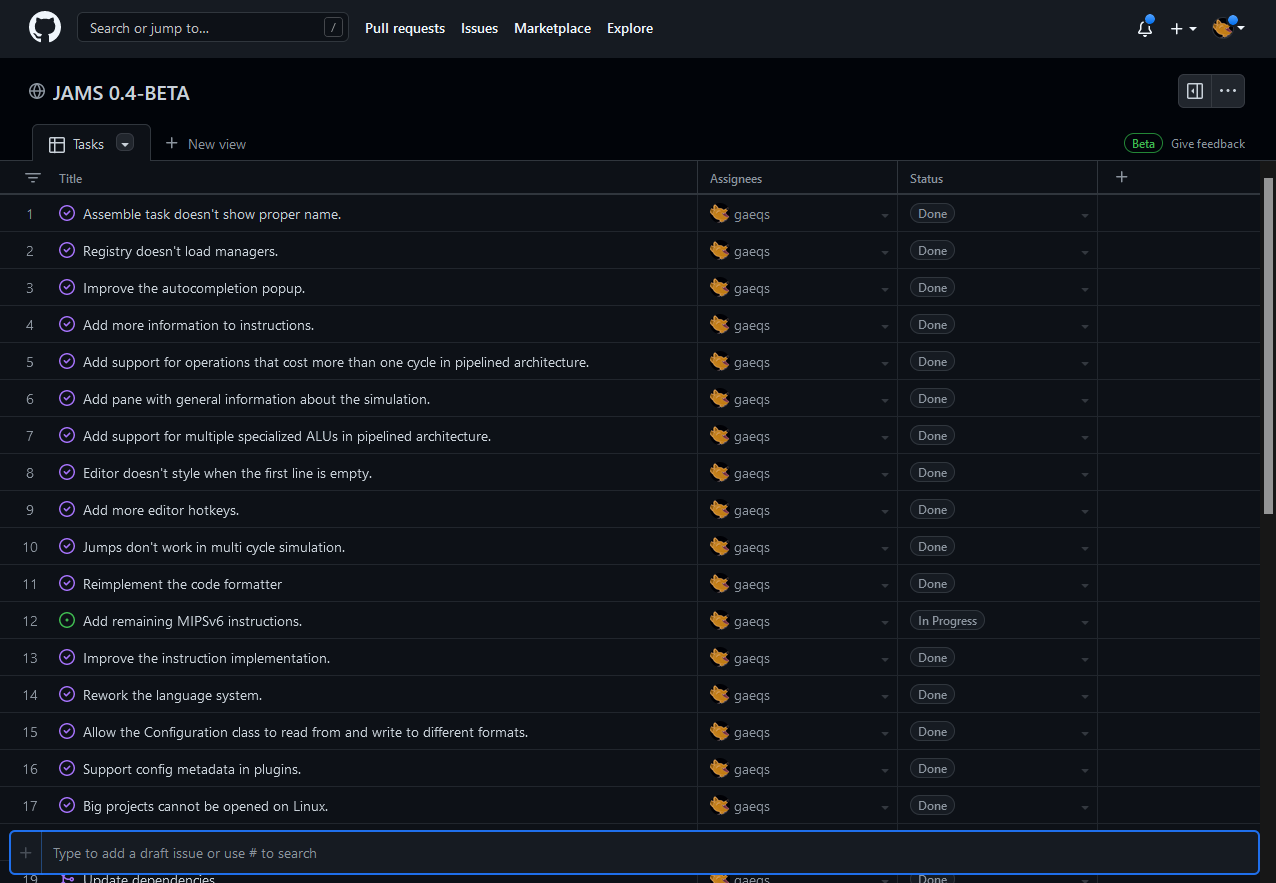
\includegraphics[width=\textwidth]{images/introduction/github}
    \caption{Proyecto de \textit{GitHub} para la versión 0.4-BETA}
    \label{fig:introduccion-github}
\end{figure}

    \chapter{Desarrollo del entorno base}\label{ch:desarrollo-del-entorno-base}

En este capítulo se abordará el desarrollo de la aplicación base, empezando por la investigación
de tecnologías.
También se definirá la estructura final de la aplicación en los ámbitos de la interfaz y el código.


\section{Definición de los requisitos de las tecnologías candidatas}
\label{sec:definicion-requisitos-tecnologías-candidatas}

Actualmente, existe una gran variedad de librerías y \textit{frameworks} gráficos que permiten
crear aplicaciones de una manera rápida y sencilla.
Estas tecnologías se pueden clasificar dependiendo de una gran cantidad de criterios.

\noindent Según su nivel de abstracción:
\begin{itemize}
    \item \textbf{Librerías de bajo nivel:} son más cercanas al \textit{hardware} gráfico.
    Permiten tener un gran control sobre los gráficos, pero no son adecuadas para
    interfaces gráficas de usuarios.
    Algunos ejemplos de librerías de bajo nivel son \textit{OpenGL}, \textit{Vulkan} o \textit{DirectX}.
    \item \textbf{Librerías de alto nivel}: incorporan una capa de abstracción sobre el \textit{hardware} gráfico.
    Permiten generar interfaces gráficas de usuario mediante una arquitectura ya definida.
    Algunos ejemplos de librerías de alto nivel son \textit{Qt}, \textit{JavaFX}, \textit{Swing}, \textit{GTK} o
    \textit{Compose Multiplatform}.
\end{itemize}

\noindent Según su disponibilidad en varias plataformas:
\begin{itemize}
    \item \textbf{Librerías exclusivas:} son librerías que solo están disponibles en una plataforma.
    Algunos ejemplos de librerías exclusivas son \textit{Windows Forms} y \textit{DirectX} en \textit{Windows},
    \textit{Metal} y \textit{QuickDraw} en \textit{MacOS} o \textit{AndroidX/Graphics} y \textit{Jetpack Compose}
    en \textit{Android}.
    \item \textbf{Librerías multiplataforma:} están disponibles en una gran variedad de plataformas.
    Algunos ejemplos de librerías multiplataforma son \textit{Qt}, \textit{JavaFX}, \textit{Swing}, \textit{GTK}
    o \textit{Compose Multiplatform}.
\end{itemize}

\noindent Un aspecto muy importante al elegir candidatos es el \textbf{lenguaje de programación}
en el que las librerías están disponibles.
Las librerías de bajo nivel suelen estar disponibles en una gran variedad de lenguajes, mientras que las
librerías de alto nivel suelen incorporar paradigmas propios del lenguaje de programación en el que están
desarrolladas.

\noindent Para el desarrollo de la aplicación se desea utilizar una librería gráfica \textbf{moderna},

\textbf{de alto nivel} y \textbf{multiplataforma}, disponible en un lenguaje de programación estable,
con una comunidad grande y \textbf{rápido tanto en el desarrollo como en la ejecución}.
Otro requisito crucial es que el lenguaje permita \textbf{vincular código externo} de manera
sencilla.

\noindent Estos requisitos reduce la lista de tecnologías en los siguientes candidatos:
\begin{itemize}
    \item \textbf{HTML, CSS y TypeScript:} este conjunto de tecnologías es muy popular actualmente
    para la creación de aplicaciones web y de escritorio. \textit{IDEs} muy famosos como
    \textit{Visual Studio Code} están desarrollados con estas tecnologías.
    \item \textbf{Kotlin / Compose Multiplatform:} \textit{Compose Multiplatform} es una librería gráfica
    para \textit{Kotlin}, un lenguaje de programación muy joven y potente que tiene el respaldo de
    grandes compañías como \textit{JetBrains} y \textit{Google}.
    \item \textbf{Java / JavaFX:} \textit{JavaFX} puede considerarse la evolución natural de \textit{Swing},
    la herramienta principal para el desarrollo de aplicaciones gráficas basadas en \textit{Java}.
    \textit{JavaFX} es una librería moderna y rápida que, gracias a que está desarrollada en \textit{Java},
    puede ser empleada por otros lenguajes de programación que corren sobre la \textit{JVM}
    \footnote{\textit{Java Virtual Machine}}, como es el caso de \textit{Scala}, \textit{Groovy} o el ya mencionado
    \textit{Kotlin}.
\end{itemize}

\noindent El trío \textit{HTML / CSS / TypeScript} suele ser una buena elección para editores y otras
aplicaciones ligeras, pero la falta de velocidad en la ejecución y la falta de consistencia por estar
basado \textit{TypeScript} en \textit{JavaScript} descarta esta opción por parte del simulador.

\noindent \textit{Kotlin / Compose Multiplatform} es una elección muy sólida actualmente, pero esta
tecnología seguía en fase \textit{beta} cuando este proyecto empezó, por lo que también ha quedado
descartada.

\noindent Finalmente, \textbf{se ha optado por utilizar el par de tecnologías \textit{Java / JavaFX}}
para el desarrollo de la aplicación, ya que cumple con todos los requisitos: \textit{Java} es un
lenguaje de programación muy estable, multiplataforma y rápido tanto en la ejecución como en
el desarrollo.
También es el lenguaje de programación con la comunidad de desarrolladores más grande.
\textit{JavaFX} es una alternativa moderna a \textit{Swing} que permite desarrollar aplicaciones
fácilmente personalizables que se alejan del ya conocido estilo de interfaz \textit{Java}.

\noindent Centrándose en otras tecnologías necesarias, se ha utilizado el entorno de desarrollo
\textit{Intellij IDEA} y el sistema de automatización \textit{Gradle} para la construcción
del proyecto.

\subsection{En defensa de \textit{Java}}\label{subsec:en-defensa-de-java}

Muchos desarrolladores piensan que \textit{Java} es un lenguaje de programación verboso, lento, pesado
y con el único propósito de crear aplicaciones \textit{Spring}.
Que la mayoría de aplicaciones \textit{Java} estén desarrolladas en versiones \textit{vanilla}
\footnote{Estándar, sin modificar} de \textit{Swing} y en versiones de \textit{Java} de hace más
de un lustro no ayuda en su reputación.

\noindent La realidad es muy diferente: su equipo de desarrollo lleva años reinventando su tecnología,
con nuevas características que acercan a \textit{Java} a lenguajes de programación mucho más modernos.
La velocidad de ejecución también se ha incrementado considerablemente, posicionándose en uno de los
lenguajes de programación que más rápido ejecutan.

\noindent Un gran ejemplo del drástico cambio que ha sufrido \textit{Java} en los últimos años son los
\textit{records}: clases de datos que son inmutables.

\begin{lstlisting}[language=Java,style=java,frame=single,label={lst:java-comparacion-18}]
public record Cat(String name, UUID owner) {
}
\end{lstlisting}

\noindent El código equivalente en \textit{Java} 8 sería el siguiente:

\begin{lstlisting}[language=Java,style=java,frame=single,label={lst:java-comparacion-8}]
public final class Cat {
    private final String name;
    private final UUID owner;

    public Cat(String name, UUID owner) {
        this.name = name;
        this.owner = owner;
    }

    public String name() { return name; }

    public UUID owner() { return owner; }

    @Override
    public boolean equals(Object obj) {
        if (obj == this) return true;
        if (obj == null || obj.getClass() != this.getClass()) return false;
        var that = (Cat) obj;
        return Objects.equals(this.name, that.name) &&
                Objects.equals(this.owner, that.owner);
    }

    @Override
    public int hashCode() { return Objects.hash(name, owner); }

    @Override
    public String toString() { return "Cat[" + "name=" + name
        + ", " + "owner=" + owner + ']'; }

}
\end{lstlisting}

\noindent La nueva arquitectura basada en módulos que presenta las librerías de \textit{Java}
ayuda mucho en la distribución de aplicaciones de escritorio, pudiendo generar un instalador
convencional que instala la aplicación junto con una versión local de la \textit{JVM} que no
suele superar los 30 MB\cite{JPACKAGE}.
Gracias a este sistema de distribución, la aplicación podrá contar con versiones
de \textit{Java} actuales sin que los usuarios tengan que pasar por complejas instalaciones.

\noindent Como dato final, existen muchas aplicaciones que se ejecutan sobre la \textit{JVM}
sin que el usuario se de cuenta.
Este es el caso de todos los \textit{IDEs} desarrollados por \textit{JetBrains}, los cuales
usan la librería \textit{Swing} con un estilo avanzado.

\begin{figure}[H]
    \centering
    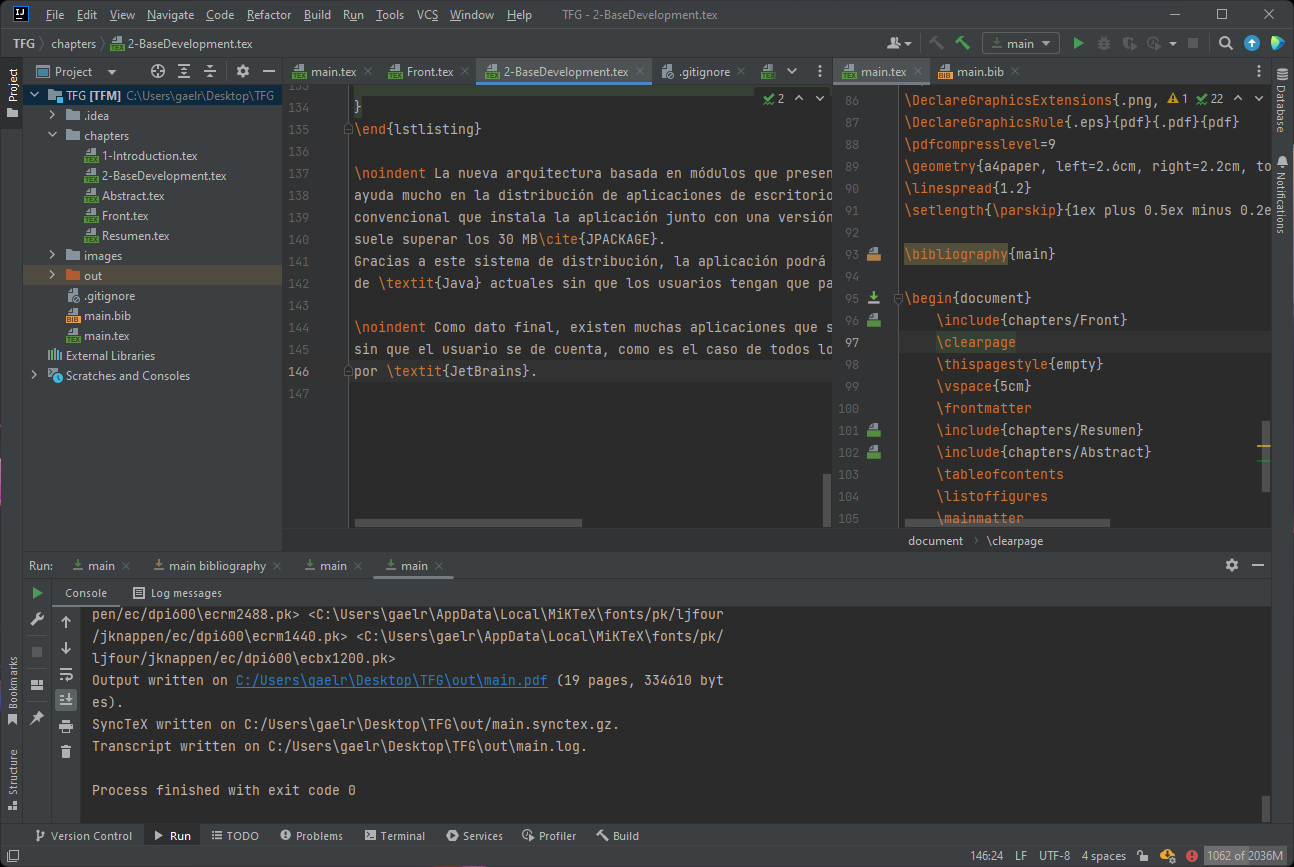
\includegraphics[width=\textwidth]{images/base/intellij-idea}
    \caption{\textit{Intellij IDEA}}
    \label{fig:java-intellij-idea}
\end{figure}


\section{Estructura del proyecto}\label{sec:estructura-del-proyecto}

\textit{JAMS} sigue los estándares de estructura de \textit{Gradle}\cite{GRADLE_ORGANIZING}.
Esto hace que su estructura sea muy similar a otras aplicaciones que usan el mismo
sistema de automatización.

\subsection{Tareas}\label{subsec:tareas}

\noindent El elemento más importante del directorio raíz es el archivo \textbf{build.gradle}.
En él se especifican las dependencias y se define cómo el proyecto debe ser compilado.
Las \textbf{tareas} son las encargadas de definir dicho comportamiento.

\noindent Las dos tareas más importantes son las siguientes:
\begin{itemize}
    \item \textbf{jpackage:} permite generar un instalador de la aplicación específico
    para la máquina que ejecuta la tarea.
    \item \textbf{bundle:} genera un archivo \textit{jar} con la aplicación y todas
    sus dependencias.
    Este archivo puede ser ejecutado en cualquier sistema operativo que pueda correr
    \textit{Java} y esté soportado por \textit{JavaFX}.
\end{itemize}

\noindent Para ejecutar estas tareas ha de usarse el \textit{script} $gradlew$.
Este comando descargará \textit{Gradle} si es necesario y ejecutará
la tarea pasada como argumento.
Todos estos comportamientos están automatizados en \textit{GitHub}
mediante los \textit{scripts} dentro de la carpeta $.github$.

\subsection{Módulos y paquetes}\label{subsec:modulos-y-paquetes}

Dentro de la carpeta $src$ están definidos los dos módulos principales del
proyecto: $main$ y $test$.

\noindent El módulo $main$ es el encargado de almacenar todo el código fuente
de la aplicación.
Puede ser considerado el módulo más importante de todo el proyecto.
El módulo $test$ define todas las pruebas unitarias que el módulo $main$
debe superar para que la aplicación se compile con éxito.

\noindent El código fuente almacenado en el módulo $main$ está separado en diferentes
paquetes \textit{Java}:
\begin{itemize}
    \item \textbf{collection:} contiene una serie de colecciones modificadas.
    \item \textbf{configuration:} contiene el sistema de configuraciones.
    \item \textbf{event:} contiene el sistema de eventos.
    \item \textbf{file:} contiene los tipos de archivo definidos en la aplicación.
    \item \textbf{gui:} contiene toda la interfaz de la aplicación.
    \item \textbf{language:} contiene el sistema de idiomas.
    \item \textbf{manager:} contiene el sistema de gestores.
    \item \textbf{mips:} contiene todas las herramientas relacionadas con la arquitectura \textit{MIPS32}.
    \item \textbf{plugin:} contiene el sistema de componentes.
    \item \textbf{project:} contiene el sistema de proyectos.
    \item \textbf{task:} contiene el sistema de hijos y tareas asíncronas.
    \item \textbf{utils:} contiene clases útiles utilizadas por los anteriores paquetes.
\end{itemize}


\section{Proyectos}\label{sec:interfaz-grafica}

\textit{JAMS} es un \textit{IDE} basado en \textbf{proyectos}.
Un proyecto está formado por una carpeta y las siguientes propiedades:
\begin{itemize}
    \item \textbf{Tipo de proyecto:} especifica el tipo de proyecto.
    En una versión sin componentes este valor solo puede tomar el valor \textit{MIPS}.
    \item \textbf{Propiedades del proyecto:} parámetros necesarios por el tipo de proyecto.
    Configuran aspectos concretos y generales de todo el proyecto.
    \item \textbf{Archivos a ensamblar:} lista de archivos que el ensamblador tendrá en cuenta
    al ensamblar el proyecto.
    \item \textbf{Configuraciones:} especifican propiedades \textbf{de una ejecución} del proyecto.
    Es decir, configuran el simulador.
    Un proyecto puede tener varias configuraciones, y el usuario ha de elegir una al crear una
    simulación.
\end{itemize}

\noindent Los proyectos son almacenados en carpetas.
Una carpeta de un proyecto tiene la siguiente estructura:

\begin{center}
    \basictree{
        [MyProject
        [.jams
        [data.json]
        [files\_to\_assemble.json]
        ]
        [Simulation Files
        [MySimulationFile.txt]
        ]
        [MyAsmFile.asm]
        ]
    }
\end{center}

\noindent Cada proyecto tiene dos carpetas por defecto: \textbf{.jams} y
\textbf{Simulation Files}.
La carpeta \textbf{.jams} contiene los datos del proyecto que \textit{JAMS}
gestiona de manera automática.
Esta carpeta está oculta y no debe ser modificada por el usuario.
El archivo \textbf{data.json} contiene el tipo de proyecto y sus propiedades,
mientras que \textit{files\_to\_assemble.json} contiene la listas de archivos
que el ensamblador ha de usar.
La carpeta \textit{Simulation Files} actúa de carpeta raíz del simulador:
todos los archivos que escriba o lea el simulador deben estar situados dentro
de esta carpeta.


\section{Gestores}\label{sec:gestores}

Toda la arquitectura de la aplicación está basada en \textbf{gestores}.
Un gestor se puede definir como un conjunto de elementos que las herramientas pueden usar.
\textit{JAMS} proporciona tres tipos básicos de gestores:
\begin{itemize}
    \item \textbf{Gestores normales:} implementados por la clase \textit{Manager}.
    Contienen una lista de elementos sin ninguna jerarquía.
    \item \textbf{Gestores con valor por defecto:} actúa como un gestor normal, con la
    diferencia que uno de sus valores es el valor por defecto.
    Estos gestores heredan de la clase \textit{DefaultValuableManager}.
    \item \textbf{Gestores con valor seleccionado:} actúan como un gestor con valor por defecto,
    pero con uno de los elementos seleccionado.
    Cuando el elemento seleccionado se elimina, el elemento por defecto queda seleccionado.
    Estos gestores heredan de la clase \textit{SelectableManager}.
\end{itemize}

\subsection{Proveedores}\label{subsec:proveedores}

Cada elemento guardado en un gestor \textbf{está asociado al proveedor que lo proporciona}.
Un proveedor puede ser un plugin o el propio \textit{JAMS}.
Cuando un proveedor se desvincula de la aplicación, todos los elementos proporcionados
por el proveedor son eliminados de los gestores.

\subsection{Registro}\label{subsec:registro}

El registro es un \textbf{elemento estático dentro de la aplicación}.
Se puede considerar un \textbf{gestor de gestores}.
En el registro se pueden recuperar, añadir, eliminar o modificar gestores.
Igual que los gestores normales, cuando un proveedor se desvincula de la aplicación,
todos los gestores proporcionados por el proveedor son eliminados del registro.

\noindent \textit{JAMS} permite separar los gestores en dos tipos:
\textbf{gestores primarios} y \textbf{gestores secundarios}.
Los gestores primarios son fácilmente accesibles cuando se busca un gestor por tipo
usando métodos como $Manager.of(Type.class)$.
Solo puede existir un gestor primario por tipo.
Para buscar gestores secundarios, se debe proveer el nombre del gestor explícitamente.

\subsection{Acceder a los gestores}\label{subsec:acceder-a-los-gestores}

Existen dos maneras de acceder a un gestor: \textbf{usando el registro} o
\textbf{usando los atajos de la clase Manager}.

\begin{lstlisting}[language=Java,style=java,frame=single,label={lst:acceder-a-los-gestores}]
// Returns the primary manager that manages languages.
Manager<Language> simpleLanguageManager = Manager.of(Language.class);
simpleLanguageManager = Jams.REGISTRY.of(Language.class);

// Returns the primary selectable manager that manages languages.
SelectableManager<Language> selectableLanguageManager = Manager.ofS(Language.class);
selectableLanguageManager = (SelectableManager<Language>) Jams.REGISTRY.of(Language.class);

// Returns the manager that is an instance of LanguageManager.
LanguageManager languageManager = Manager.get(LanguageManager.class);
languageManager = Jams.REGISTRY.get(LanguageManager.class);

// Returns the manager with the given name.
Manager<Language> manager = Jams.REGISTRY.of("other-language-manager", Language.class);
\end{lstlisting}

\subsection{Usar los gestores}\label{subsec:usar-los-gestores}

Los \textbf{gestores} implementan la interfaz $Set$
\footnote{https://docs.oracle.com/javase/8/docs/api/java/util/Set.html},
por lo que son fácilmente manipulables.

\begin{lstlisting}[language=Java,style=java,frame=single,label={lst:usar-los-gestores}]
SelectableManager<Language> manager = Manager.ofS(Language.class);

// Accessing elements
Language selectedLanguage = manager.getSelected();
Optional<Language> english = manager.get("English");

// Iterate through the manager
manager.forEach(language -> System.out.println(language.getName()));

// Adding and removing elements
if (english.isPresent()) {
    manager.remove(english.get());
    manager.add(english.get());
}
\end{lstlisting}

\subsection{Crear nuevos gestores}\label{subsec:crear-nuevos-gestores}

Se pueden crear gestores de cualquier tipo de dato que extienda la interfaz $ManagerResource$.

\begin{lstlisting}[language=Java,style=java,frame=single,label={lst:crear-nuevos-gestores}]
// The element to store inside the manager
public record MyElement(ResourceProvider provider, String name, double value) implements ManagerResource {
    @Override
    public ResourceProvider getResourceProvider() {return provider;}

    @Override
    public String getName() {return name;}
}

// The manager implementation
public class MyManager extends Manager<MyElement> {

    public MyManager(ResourceProvider provider) {
        super(provider, "my-manager", MyElement.class, false);
    }

    @Override
    protected void loadDefaultElements() {
        add(new MyElement(provider, "test-1", 1.0));
        add(new MyElement(provider, "test-2", 2.0));
        add(new MyElement(provider, "test-3", 3.0));
    }
}
\end{lstlisting}


\section{Eventos}\label{sec:eventos}

\textit{JAMS} incluye un sistema de eventos que permite informar de sucesos entre componentes de la aplicación.
Este sistema está profundamente inspirado en el sistema de eventos usado por la comunidad de \textit{Minecraft}
en proyectos como \textit{Spigot}\footnote{https://www.spigotmc.org/}
o \textit{Sponge}\footnote{https://www.spongepowered.org/}, y puede considerarse una evolución descentralizada
de esta tecnología.

\subsection{Emisores de eventos}\label{subsec:emisores-de-eventos}

Los emisores de eventos son los encargados de relacionar los creadores de eventos con sus escuchadores.
Un emisor de evento está representado por la interfaz $EventBroadcast$.
Esta interfaz es implementada por cualquier elemento que quiera ser usado para registrar escuchas.
Los gestores, los componentes, o el propio \textit{JAMS} implementan un emisor por defecto.
La clase $SimpleEventBroadcast$ contiene una implementación de $EventBroadcast$
que se puede usar como superclase.

\subsection{Definir escuchas}\label{subsec:definir-escuchas}

Las escuchas son \textbf{métodos no estáticos anotados con la anotación @Listener}.
Estos métodos solo tienen un parámetro que pide un elemento que extienda la clase
$Event$ y deben devolver $void$.

\begin{lstlisting}[language=Java,style=java,frame=single,label={lst:definir-escuchas}]
@Listener
private void onLanguageRegister(ManagerElementRegisterEvent.After<Language> event) {
    System.out.println("New language available! " + event.getElement().getName());
}
\end{lstlisting}

\noindent Este método, después de ser registrado en un gestor de idiomas,
se ejecutará cuando un nuevo idioma sea añadido al gestor.

\noindent A diferencia de otros sistemas de eventos similares,
el sistema de eventos de \textit{JAMS} permite usar \textbf{eventos genéricos}.
Un ejemplo es el caso anterior, donde el método pide un elemento de tipo
$ManagerElementRegisterEvent.After<Language>$.
Si el emisor al que está registrado emite un evento de tipo
$ManagerElementRegisterEvent.After<Theme>$, la escucha no será invocada.

\noindent Un evento puede extender la clase de otro evento.
Esto permite generar una jerarquía de eventos.
Una escucha que pide un cierto tipo de evento se ejecutará siempre que dicho evento o uno de sus hijos ocurra.
Si una escucha pide el evento $Event$, su método se ejecutará siempre que un evento ocurra.

\noindent Algunos eventos implementan la interfaz $Cancellable$, lo cual permite cancelar el evento.
Las escuchas restantes no serán llamadas cuando un evento es cancelado salvo que se defina lo contrario
en la etiqueta $@Listener$.

\subsection{Registrar escuchas}\label{subsec:registrar-escuchas}

Una vez se tenga una escucha definida, esta se puede registrar en uno o varios emisores de eventos.
Al ser las escuchas no estáticas, toda escucha registrada en un emisor está ligada al evento con el
que debe ser invocado.
Esto añade una gran flexibilidad al sistema, permitiendo que un elemento registre
escuchas dependiendo de su estado.

\noindent El método más usado para registrar escuchas es el método
$registerListeners(Object, boolean)$.
Este método buscará en el objeto todos los métodos con la etiqueta $@Listener$
que pidan un evento y devuelvan $void$.
Esta búsqueda incluye a todos los métodos definidos en el objeto,
incluyendo métodos privados y métodos de las superclases.

\noindent El booleano $useWeakReferences$ permite registrar la escucha usando una referencia débil.
Si este booleano es falso, el objeto usado para el registro quedará en memoria aunque todas
sus referencias cesen de existir, por lo que se debe eliminar el registro de manera manual.
La referencia débil elimina este paso, borrándose el registro automáticamente cuando
el elemento deja de ser referenciado.

\begin{lstlisting}[language=Java,style=java,frame=single,label={lst:registrar-escuchas}]
private void register() {
    Manager<Language> manager = Manager.of(Language.class);
    manager.registerListeners(this, true);
}

@Listener
private void onLanguageRegister(ManagerElementRegisterEvent.After<Language> event) {
    System.out.println("New language available! " + event.getElement().getName());
}
\end{lstlisting}

\noindent Si se desea, se puede registrar una única escucha del objeto.
Este método requiere conocimientos de la librería \textit{reflection} de \textit{Java}:

\begin{lstlisting}[language=Java,style=java,frame=single,label={lst:registrar-escuchas-2}]
private void register() throws NoSuchMethodException {
    Manager<Language> manager = Manager.of(Language.class);
    manager.registerListener(
            this,
            this.getClass().getDeclaredMethod("onLanguageRegister", ManagerElementRegisterEvent.class),
            true
    );
}

@Listener()
private void onLanguageRegister(ManagerElementRegisterEvent.After<Language> event) {
    System.out.println("New language available! " + event.getElement().getName());
}
\end{lstlisting}

\noindent Para eliminar los registros, se han de usar los métodos análogos
$unregisterListeners$ y $unregisterListener$.

\subsection{Parámetros avanzados}\label{subsec:parámetros-avanzados}

La etiqueta $@Listener$ permite definir comportamientos más avanzados en la escucha.

\begin{lstlisting}[language=Java,style=java,frame=single,label={lst:escuchas-avanzadas}]
@Listener(priority = 20, ignoreCancelled = true)
private void onLanguageRegister(ManagerElementRegisterEvent.After<Language> event) {
    System.out.println("New language available! " + event.getElement().getName());
}
\end{lstlisting}

\noindent El parámetro $priority$ permite definir la prioridad de la escucha.
La escucha con el número más alto será la primera en ser llamada.
El parámetro $ignoreCancelled$ es un booleano que le da a la escucha la capacidad
de ser llamada incluso cuando un evento ha sido cancelado.


\section{Interfaz de usuario}\label{sec:interfaz-de-usuario}

La interfaz de \textit{JAMS} es muy similar a las interfaces que presentan los \textit{IDEs} modernos.
Todas las herramientas están encapsuladas en $nodos$.
Cada nodo se puede desplegar en los laterales del editor.
Más concretamente, se pueden desplegar dos nodos por cada lado del editor.

\begin{figure}[H]
    \centering
    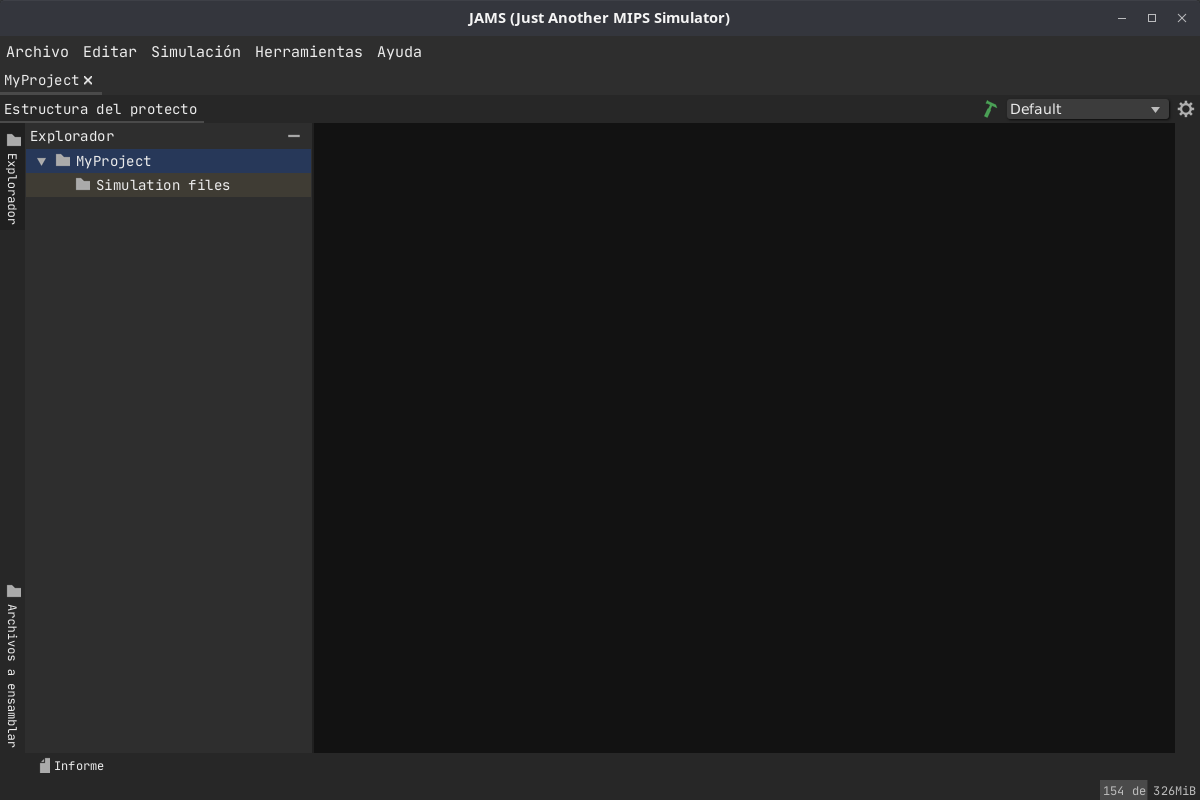
\includegraphics[width=0.8\textwidth]{images/base/jams-basic}
    \caption{\textit{Editor de \textit{JAMS} en su forma más básica}}
    \label{fig:jams-basic}
\end{figure}

\noindent Los nodos también se pueden configurar para que se desplieguen en una ventana aparte.
Esto permite poder desplegar un número indefinido de nodos al mismo tiempo.
El modo de despliegue se puede configurar presionando el botón secundario sobre
el botón del nodo.

\begin{figure}[H]
    \centering
    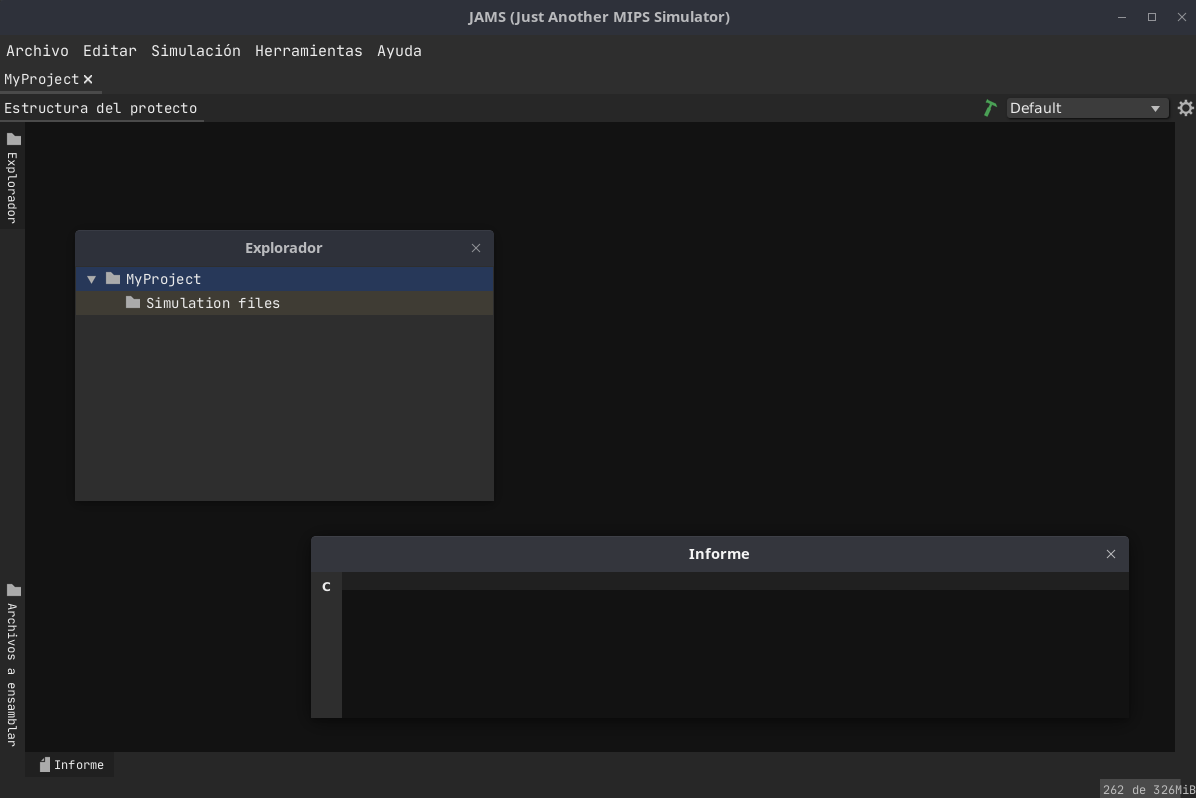
\includegraphics[width=0.8\textwidth]{images/base/jams-windows}
    \caption{\textit{Editor de \textit{JAMS} con ventanas desplegadas}}
    \label{fig:jams-windows}
\end{figure}

\subsection{Menú superior}\label{subsec:menu-superior}

El menú superior de \textit{JAMS} funciona de manera idéntica a cualquier otro programa.
Por defecto existen cinco secciones:
\begin{itemize}
    \item \textbf{Archivo}: permite crear o abrir nuevos proyectos, además de
    acceder a la configuración.
    \item \textbf{Editar:} permite acceder a los comandos del editor de texto.
    \item \textbf{Simulación:} permite acceder a los comandos de simulación.
    \item \textbf{Herramientas:} permite habilitar o deshabilitar nodos.
    \item \textbf{Ayuda:} permite acceder a ayuda sobre \textit{JAMS}.
\end{itemize}

\subsection{Proyectos abiertos}\label{subsec:proyectos-abiertos}

Los proyectos abiertos aparecen justo debajo del menú superior.
Cada proyecto está representado por una pestaña, lo que facilita alternar entre
proyectos abiertos.
Si se cierran todos los proyectos, \textit{JAMS} cerrará el editor y trasladará
al usuario a la ventana de inicio.

\noindent Los proyectos presentan una lista de pestañas con todas las secciones
que tienen abiertas.
Normalmente, la primera pestaña representa el editor del proyecto, mientras que
las siguientes representan las simulaciones que el usuario vaya creando.

\begin{figure}[H]
    \centering
    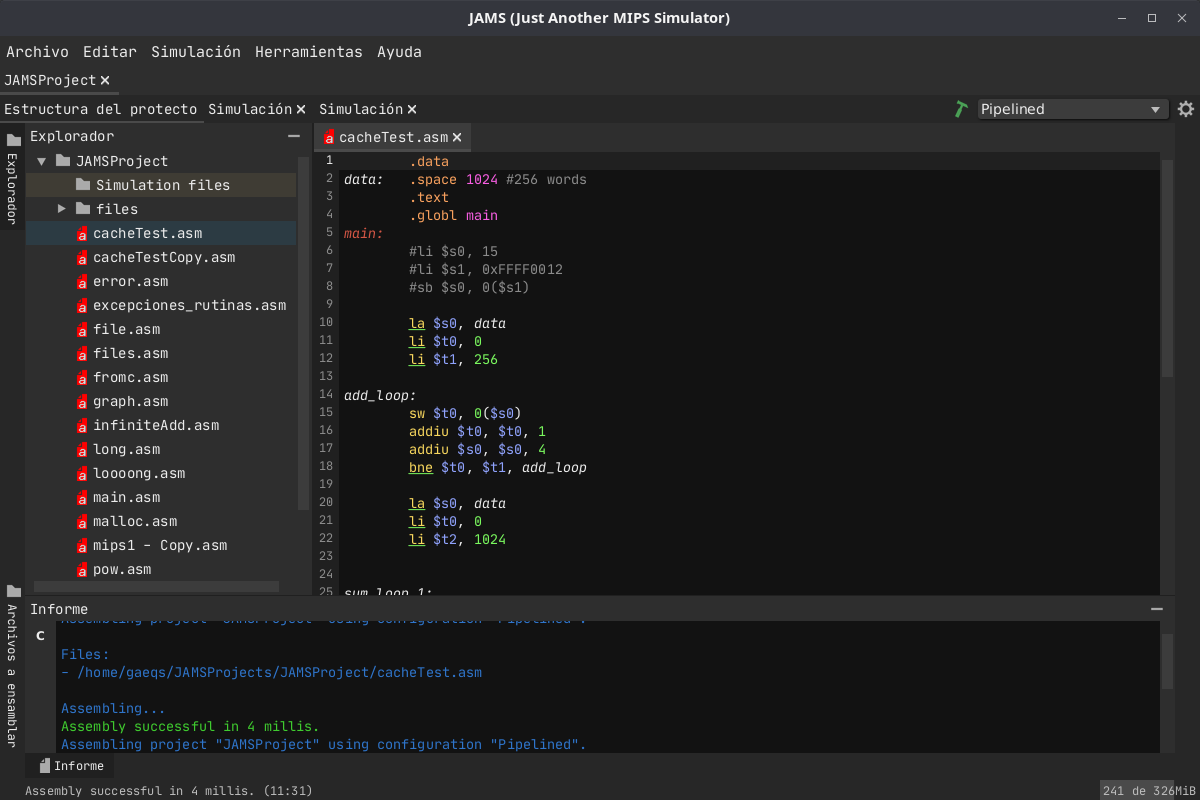
\includegraphics[width=0.8\textwidth]{images/base/jams-sections}
    \caption{\textit{Editor de \textit{JAMS} con varias simulaciones creadas}}
    \label{fig:jams-sections}
\end{figure}

\noindent Cada sección tiene una \textbf{barra de herramientas} propia.
Esta barra está situada a la izquierda de la lista de secciones, y permite
ejecutar acciones relacionadas con la sección actual.

\subsection{Barra inferior}\label{subsec:barra-inferior}

La barra inferior del editor es común a todas las secciones.
En esta, se informa del último mensaje escrito en el \textbf{informe}.
A la izquierda también se muestra la memoria que está usando actualmente
\textit{JAMS}.
Al estar creada la aplicación en \textit{Java}, esta utiliza un recolector
de basura.
Se puede forzar el paso del recolector de basura pulsando el panel que informa
sobre el uso de memoria.

\subsection{Ventana principal}\label{subsec:ventana-principal}

Si \textit{JAMS} no tiene ningún proyecto que mostrar, se mostrará la ventana
principal.
En esta ventana se pueden encontrar cuatro apartados:
\begin{itemize}
    \item \textbf{Proyectos:} en este apartado se encuentran los proyectos más
    recientes.
    También se puede abrir un proyecto ya existente.
    \item \textbf{Nuevo proyecto:} este apartado permite crear nuevos proyectos.
    Un componente puede añadir su propio creador de proyectos.
    \item \textbf{Configuración:} muestra la ventana de configuración.
    Permite configurar \textit{JAMS} antes de abrir un proyecto.
    \item \textbf{Acerca de:} muestra información básica sobre \textit{JAMS}.
\end{itemize}

\begin{figure}[H]
    \centering
    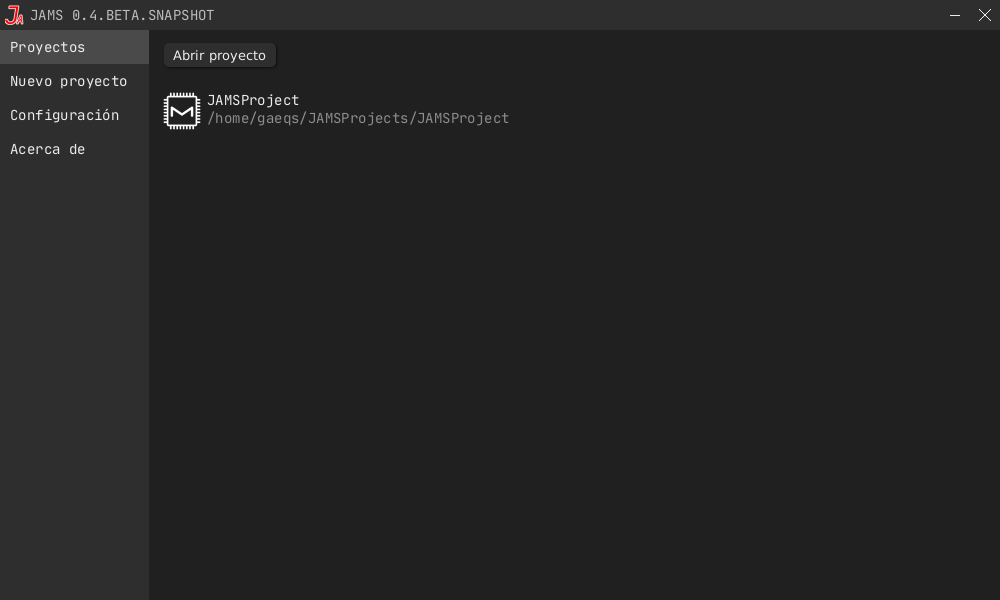
\includegraphics[width=0.8\textwidth]{images/base/jams-main-projects}
    \caption{\textit{Ventana principal mostrando los proyectos recientes}}
    \label{fig:jams-main-projects}
\end{figure}

\begin{figure}[H]
    \centering
    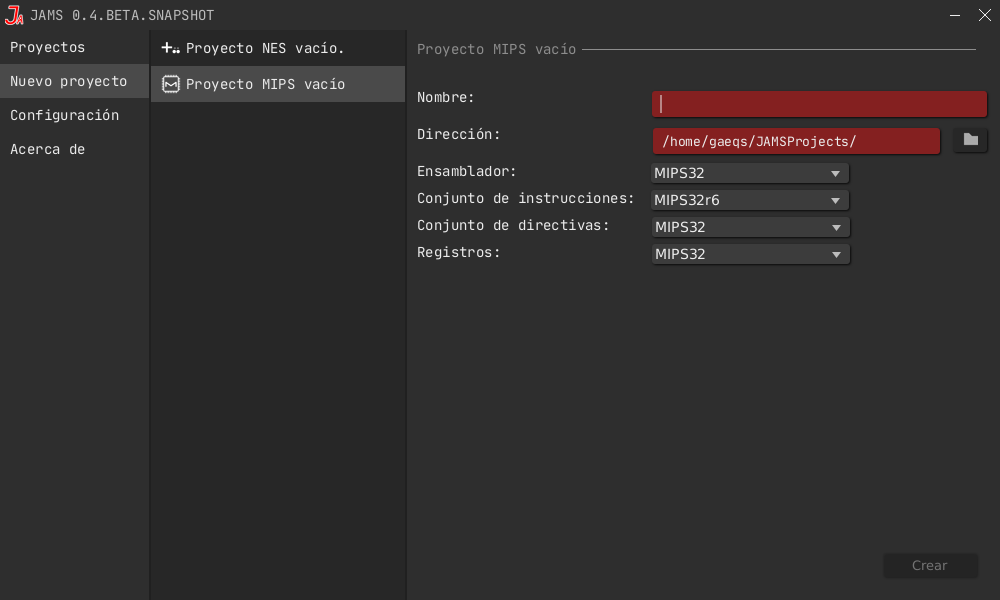
\includegraphics[width=0.8\textwidth]{images/base/jams-main-new-project}
    \caption{\textit{Ventana de creación de nuevos proyectos}}
    \label{fig:jams-main-new-project}
\end{figure}


\section{Idiomas}\label{sec:idiomas}

Igual que cualquier aplicación moderna, \textit{JAMS} presenta un sistema de
localización basado en paquetes de idiomas.
Cualquier usuario o componente puede crear un paquete que añada
o modifique un idioma.

\subsection{Estructura de un paquete}\label{subsec:estructura-de-un-paquete}

Un paquete de idiomas es una carpeta o un archivo comprimido
que contienen un archivo \textbf{language.json} y varios archivos \textit{YAML}.
Esta carpeta o archivo estará situado dentro de un componente
o dentro de la carpeta \textbf{~/JAMS/languages}.
Un ejemplo de un archivo \textbf{language.json} sería el siguiente:

\begin{lstlisting}[frame=single,label={lst:language.json}]
{
  "name": "English",
  "priority": 0,
  "files": [
    "actions.yml",
    "configuration.yml",
    "directives.yml",
    "editor.yml",
    "general.yml",
    "instructions.yml",
    "interface.yml",
    "mips_elements.yml",
    "mips_simulation_configuration.yml",
    "simulation.yml"
  ]
}
\end{lstlisting}

\noindent Dentro de este archivo se encuentran los siguientes parámetros:
\begin{itemize}
    \item \textbf{name:} es el nombre del idioma.
    Este nombre es el que será mostrado al usuario
    y actúa como identificador del idioma.
    \item \textbf{files:} son los archivos \textit{YAML} que componen el paquete.
    \item \textbf{priority:} es la prioridad del paquete si existen varios
    paquetes para el mismo idioma.
    Cuanto más alto sea el número, más prioridad tiene el paquete.
    Esta propiedad es opcional y por defecto toma el valor 0.
\end{itemize}

\noindent Los archivos \textit{YAML} pueden estar en carpetas dentro del paquete,
y deben estar definidos en el archivo \textbf{language.json} con una
dirección relativa a la raíz del paquete.
Un ejemplo de archivo \textit{YAML} sería el siguiente:

\begin{lstlisting}[frame=single,label={lst:interface.yml}]
START_TITLE: JAMS {VERSION}
START_PROJECTS: Projects
START_NEW_PROJECT: New project
START_ABOUT: About
BOTTOM_BAR_MEMORY: '{USED} of {TOTAL}MiB'
BOTTOM_BAR_MEMORY_TOOLTIP: Click to execute the garbage collector.

MAIN_MENU_FILE: File
MAIN_MENU_EDIT: Edit
MAIN_MENU_SIMULATION: Simulation
MAIN_MENU_TOOLS: Tools
MAIN_MENU_HELP: Help
MAIN_MENU_FILE_EXIT: Exit
MAIN_MENU_FILE_SETTINGS: Settings
MAIN_MENU_FILE_OPEN_PROJECT: Open project
MAIN_MENU_FILE_CREATE_PROJECT: Create project
MAIN_MENU_FILE_CREATE_PROJECT_TITLE: Create project
MAIN_MENU_FILE_CREATE_PROJECT_NAME: 'Name:'
MAIN_MENU_FILE_CREATE_PROJECT_PATH: 'Path:'
MAIN_MENU_HELP_ABOUT: About
\end{lstlisting}

\noindent Aunque no se use en ningún paquete por defecto,
los paquetes de idiomas permiten crear secciones como
en cualquier archivo \textit{YAML}.
En el siguiente caso, se usará el identificador
$ACTION.MY\_ACTION$ para referenciar el mensaje.

\begin{lstlisting}[frame=single,label={lst:yaml-subsection}]
ACTION:
  MY_ACTION: My action
\end{lstlisting}

\subsection{Extensiones}\label{subsec:idiomas-extensiones}

Puede existir el caso donde varios paquetes hagan referencia al mismo idioma.
Este problema de colisión se soluciona gracias a las extensiones.
Un paquete actúa siempre como una extensión de un idioma.
Esta extensión tiene una prioridad que se define en el archivo
\textbf{language.json} del paquete.
Si dos extensiones tienen la misma prioridad, el orden se resuelve
por orden de creación de la extensión, siendo el último en ser creado
el que tenga más prioridad.
El mensaje ligado a un identificador será el de la extensión con más prioridad
que contenga un mensaje ligado al identificador.
Gracias a este pequeño sistema de extensiones, los usuarios podrán crear modificaciones
y los componentes podrán añadir nuevos mensajes.

\subsection{Acceder a mensajes}\label{subsec:acceder-a-mensajes}

Existen dos maneras de acceder a los mensajes mediante un identificador:
\textbf{de manera directa} o \textbf{usando un componente preparado}.

\noindent Un componente puede acceder al idioma seleccionado usando
el gestor de idiomas por defecto.
La manera más correcta para pedir un mensaje es usando el método
$getOrDefault(String)$ del idioma.
Este método devolverá el mensaje asociado al identificador dado.
Si el idioma no contiene ningún mensaje con ese identificador,
lo buscará en el idioma por defecto.
Si ninguno de los dos idiomas contiene el mensaje,
devuelve una cadena de texto vacía.

\noindent Cabe destacar que esta acción suele deber rehacerse cuando
el idioma cambia, por lo que se debe registrar una escucha en el
gestor de idiomas, escuchando el evento $LanguageRefreshEvent$.
Si esto no se hace, el seguirá mostrando el mensaje en el idioma
anterior.

\begin{lstlisting}[language=Java,style=java,frame=single,label={lst:idioma-escucha}]
@Listener
public void onRefresh(LanguageRefreshEvent event) {
    refreshMessage(event.getSelectedLanguage());
}
\end{lstlisting}

\noindent También existe una gran variedad de nodos de \textit{JavaFX} preparados
para usar mensajes traducibles, sin necesidad de que el desarrollador tenga que
gestionar escuchas y gestores.
Estos nodos se pueden encontrar en el paquete
$net.jamsimulator.jams.language.wrapper$.

\begin{lstlisting}[language=Java,style=java,frame=single,label={lst:idioma-nodo}]
new LanguageLabel(Messages.ACTION_FOLDER_EXPLORER_ELEMENT_NEW_FOLDER)
\end{lstlisting}


\section{Temas}\label{sec:temas}

Los temas de JAMS funcionan de la misma manera que el estilo de una página web:
mediante archivos \textit{CSS}.
funcionamiento de los temas es muy similar al funcionamiento de los idiomas:
los temas son empaquetados en una carpeta o archivo comprimido,
con un archivo \textit{JSON} que actúa como punto de entrada (\textbf{theme.json})
y un conjunto de archivos \textit{CSS}.

\noindent A diferencia de los idiomas, un desarrollador que implemente nuevos
nodos a la escena de \textit{JAMS} no require gestionar ningún aspecto
de los temas: el tema que el usuario tenga seleccionado será implementado
de manera transparente gracias al sistema de temas de \textit{JavaFX}.

\subsection{Estructura}\label{subsec:estructura}

El archivo \textbf{theme.json} define el nombre y los archivos
\textit{CSS} incluidos en el tema.
Un ejemplo de archivo theme.json sería el siguiente:
\begin{lstlisting}[frame=single,label={lst:theme.json}]
{
  "name": "Light Theme",
  "dependencies": ["Other Theme"],
  "files": [
    "extra.css"
  ]
}
\end{lstlisting}

\noindent Un archivo \textbf{theme.json} presenta los siguientes parámetros:
\begin{itemize}
    \item \textbf{name:} es el nombre del tema.
    Este nombre es el que será mostrado al usuario
    y actúa como identificador del tema.
    \item \textbf{files:} son los archivos \textit{CSS} que componen el paquete.
    \item \textbf{dependencies:} los temas de los que este tema depende.
    El estilo de estos temas será añadido al estilo del tema definido.
    Este parámetro es opcional.
\end{itemize}

\noindent Estén definidos o no las dependencias,
todo tema depende del tema $Common$.
Este tema actúa de base, y define el estilo básico de \textit{JAMS}.
Este tema define muchas variables globales, pero no le asigna ningún
valor a ninguna de ellas.

\subsection{Variables globales}\label{subsec:variables-globales}

Las variables globales permiten definir el color de los diferentes
componentes de manera muy sencilla.
Un tema debe asignar un color a todas las variables del tema $Common$.
Esta tarea se debe hacer en el archivo especial \textbf{global.css}.
Este archivo es un archivo especial que siempre está incluido en el tema y,
al compilar, será envuelto en una sección global \textit{CSS} $*\{ \}$.
Esto permite que todos los componentes puedan usar
las variables asignadas en este archivo.
Un ejemplo de archivo \textbf{global.css} sería el siguiente:

\begin{lstlisting}[frame=single,label={lst:global.css}]
-theme-foreground: #222222;
-theme-foreground-darker: derive(-theme-foreground, 20%);
-theme-foreground-darker-2: derive(-theme-foreground, 40%);
-theme-foreground-lighter: #000000;
-theme-background: #f2f2f2;
-theme-background-darker: #e5e5e5;
-theme-background-darker-2: #eaeaea;
-theme-background-lighter: #f7f7f7;
-theme-background-pressed: derive(-theme-background, -10%);
-theme-background-darkest: #FFFFFF;
-theme-shadow: #555555;
-theme-header: #8faccc;
-theme-menu-item-hover: #4D6EAF;

...
\end{lstlisting}

\subsection{Extensiones}\label{subsec:temas-extensiones}

Igual que los idiomas, los temas funcionan mediante extensiones.
Todo paquete de temas es convertido en una extensión del tema que define.
Si existen varios paquetes apuntando al mismo tema, los dos coexistirán
como dos extensiones del mismo tema.
Una gran diferencia a los idiomas es que las extensiones de los temas
no tienen prioridad.
\textit{JavaFX} sigue el estándar
\textit{CSS}\footnote{\url{https://developer.mozilla.org/en-US/docs/Web/CSS/Specificity\#how_is_specificity_calculated}}
para la prioridad de las definiciones,
por lo que una capa de prioridades más es innecesaria.

\begin{figure}[H]
    \centering
    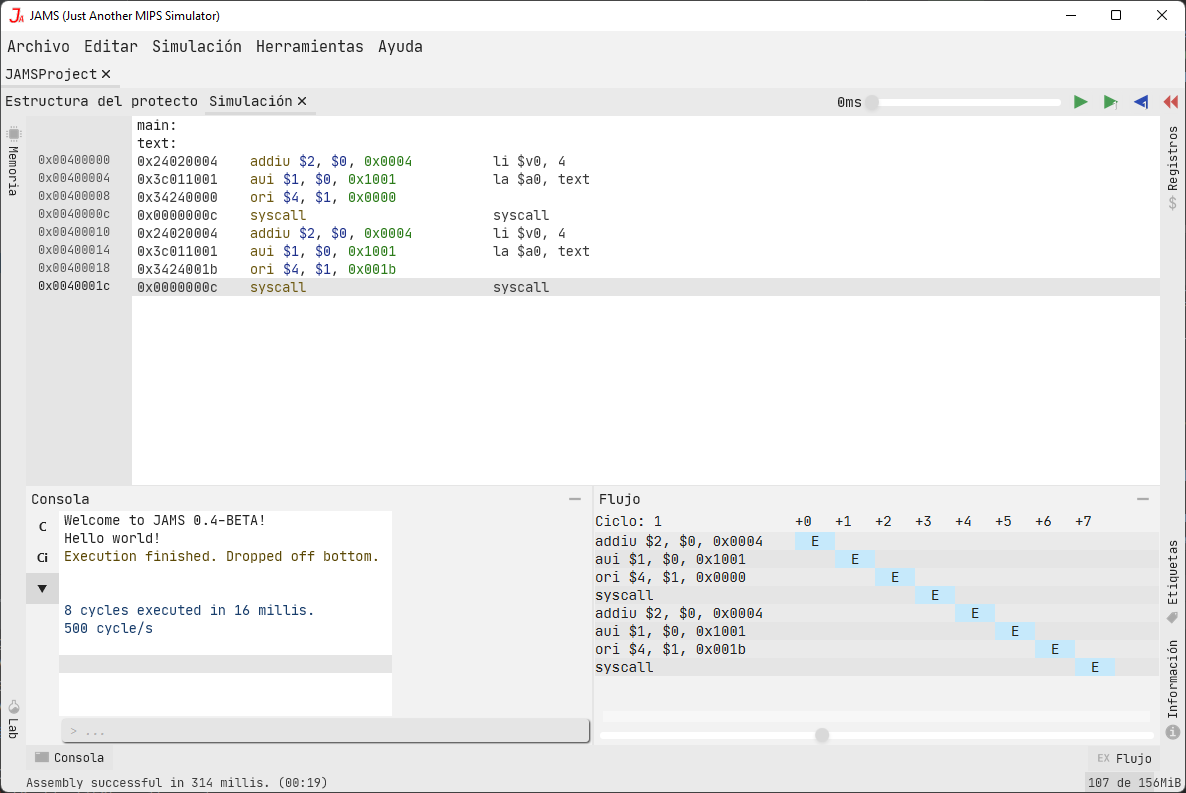
\includegraphics[width=0.8\textwidth]{images/base/jams-theme}
    \caption{\textit{JAMS} configurado para usar el modo claro}
    \label{fig:jams-registers}
\end{figure}


\section{Configuración}\label{sec:configuracion}

Igual que cualquier aplicación moderna, \textit{JAMS} presenta una
ventana de configuración donde el usuario podrá personalizar su experiencia.
Internamente, el sistema de configuraciones orbita alrededor de dos archivos \textit{JSON}:
\textbf{el archivo de valores} y el \textbf{archivo de estructura}.

\noindent El archivo de valores es el encargado de almacenar los valores de
todos los \textbf{nodos} de la configuración.
Existe dos versiones de este archivo:
el primero se encuentra en la carpeta \textbf{~/JAMS} y representa los \textbf{valores
actuales de la configuración}.
El segundo se encuentra dentro de la propia aplicación, y es el encargado de
proporcionar \textbf{los valores por defecto de cada nodo}.
Un componente podrá agregar nuevos valores a este archivo.

\begin{lstlisting}[frame=single,label={lst:main_config.json}]
{
    "language": {
        "default": "English",
        "selected": "English"
    },
    "appearance": {
        "theme": "Dark Theme",
        "hide_top_bar": false,
        "general_font": "JetBrains Mono",
        "code_font": "JetBrains Mono",
        "antialiasing": true
    },
    "editor": {
        "zoom_using_mouse_wheel": true,
        "reset_zoom_using_middle_button": true,
        "zoom_sensibility": 0.007,
        "mips": {
            "use_tabs": true,
            "preserve_tabs": true,
            "preserve_tabs_before_labels": true,
            "space_after_instruction": "SPACE",
            "space_after_instruction_parameter": "COMMA_AND_SPACE",
            "space_after_directive": "SPACE",
            "space_after_directive_parameter": "SPACE",
            "maximum_blank_lines": 2
        }
    }
}
\end{lstlisting}

\noindent El archivo de estructura o metadatos contiene información
relacionada sobre el propio nodo: el \textbf{tipo}, \textbf{región}
y \textbf{nombre} de cada nodo están definidos en este archivo.
Las secciones también tienen sus propios metadatos, especificando
el \textbf{nombre} de la sección y sus \textbf{regiones} con sus
\textbf{prioridades}.

\begin{lstlisting}[frame=single,label={lst:main_config_meta.json}]
{
    "language": {
        "meta": {
            "language_node": "CONFIG_LANGUAGE",
            "regions": {
                "language": 0
            }
        },
        "default": {
            "type": "language",
            "language_node": "CONFIG_LANGUAGE_DEFAULT",
            "region": "language"
        },
        "selected": {
            "type": "language",
            "language_node": "CONFIG_LANGUAGE_SELECTED",
            "region": "language"
        }
    }
}
\end{lstlisting}

\subsection{Interfaz de la configuración}\label{subsec:interfaz-de-la-configuración}

Para evitar que los usuarios tengan que modificar los valores de la configuración
externamente, se ha implementado una interfaz que permite modificar los
parámetros al vuelo dentro de la aplicación.
Esta interfaz es accesible directamente en la ventana de inicio o accediendo a ella
mediante la opción \textbf{Archivo > Configuración}.

\begin{figure}[H]
    \centering
    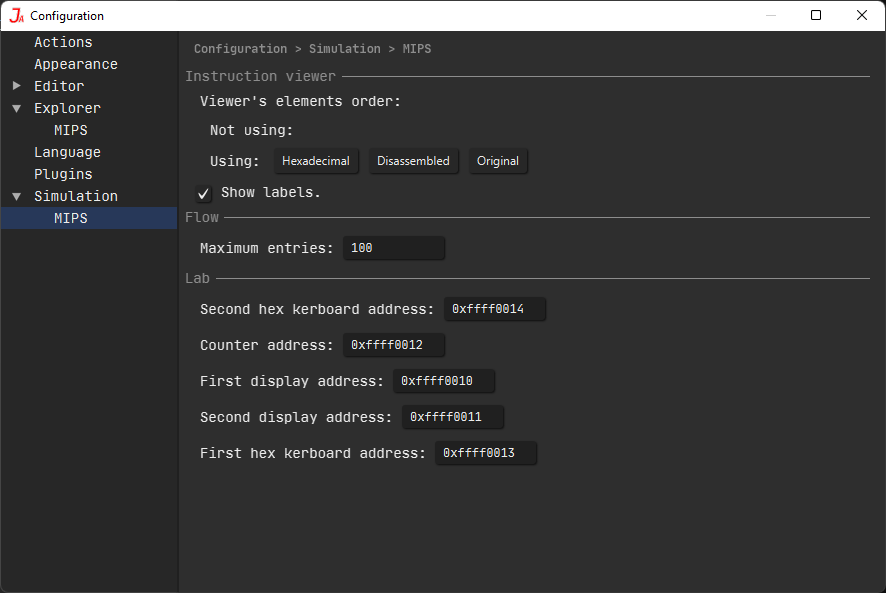
\includegraphics[width=0.8\textwidth]{images/base/jams-config}
    \caption{\textit{Interfaz de configuración}}
    \label{fig:jams-configuracion}
\end{figure}

\noindent Esta interfaz aprovecha los metadatos proporcionados por el archivo
de estructura para proporcionar una interacción adecuada entre el usuario
y los diferentes parámetros.
Esta interfaz es extensible, pudiendo los componentes añadir nuevos tipos de datos
proporcionando un $ValueEditor$ y un $ValueConverter$.
Un $ValueConverter$ permite transformar un objeto compuesto a una cadena
de caracteres y vice-versa.
Un $ValueEditor$ proporciona una interfaz de edición adecuada para un
objeto compuesto.

\subsection{Secciones especiales}\label{subsec:secciones-especiales}

La interfaz de la configuración permite que ciertas gestiones se
gestionen de manera externa por un controlador diferente al de
por defecto.
Este es el caso de las secciones \textbf{Acciones} y \textbf{Plugins}.
Estas secciones tienen una estructura totalmente diferente a la
del resto de secciones, lo que permite al usuario modificar
de manera más eficiente sus parámetros.

\begin{figure}[H]
    \centering
    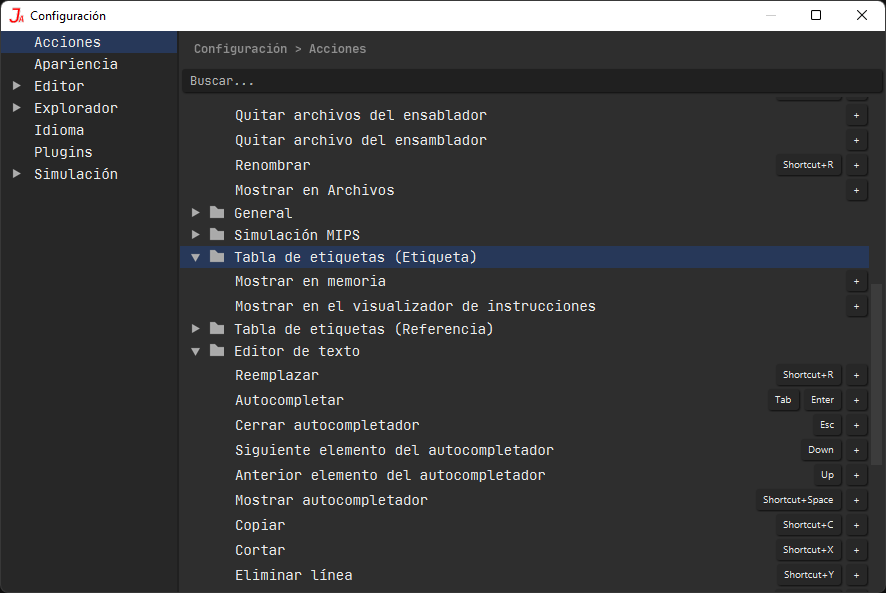
\includegraphics[width=0.8\textwidth]{images/base/jams-config-actions}
    \caption{\textit{Sección de acciones}}
    \label{fig:jams-configuracion-acciones}
\end{figure}


\section{Acciones}\label{sec:acciones}

Las acciones representan tareas que un usuario puede realizar de manera
\textbf{atómica}.
Las acciones pueden invocarse de diferentes maneras:
desde el menú principal, desde un menú de contexto
o usando una combinación de teclas modificable.
Cabe destacar que las acciones son \textbf{sensibles al contexto}:
una acción solo se podrá ejecutar en un determinado contexto
de la aplicación (el usuario no puede copiar un trozo de texto
en el explorador).

\noindent Los componentes pueden implementar nuevas acciones
creando una nueva clase que extienda $Action$ o $ContextAction$.
La clase $Action$ es la clase básica para las acciones.
Las implementaciones deben implementar el funcionamiento
de la acción en el método $run$.
La clase $ContextAction$ permite que la acción sea
mostrada en un menú contextual.
Las implementaciones de esta clase deben implementar
muchos más métodos que proporcionan información
sobre la viabilidad de la acción en diferentes contextos.


\section{Editor de texto}\label{sec:editor-de-texto}

El editor de texto es la tecnología que más iteraciones
ha sufrido en todo el desarrollo de \textit{JAMS},
siendo uno de los elementos más avanzados de toda
la aplicación.
El editor de texto presenta una arquitectura
\textbf{asíncrona}, y permite gestionar una gran
cantidad de líneas de texto sin bloquear la aplicación.

\subsection{Arquitectura}\label{subsec:arquitectura}

El editor de texto presenta una arquitectura
\textbf{Modelo-Vista-Controlador}:
\begin{itemize}
    \item \textbf{Vista:} la vista está gestionada
    por la librería \textit{RichTextFX}\cite{RICH_TEXT_FX}.
    \textit{RichTextFX} permite añadir estilos
    a secciones del texto.
    La vista está representada por la clase
    $CodeArea$.
    \item \textbf{Controlador:} el controlador está
    gestionado por la clase $CodeFileEditor$.
    Esta clase extiende $CodeArea$, y es la
    encargada de gestionar las entradas del usuario.
    \item \textbf{Modelo:} el modelo está representado
    por la clase $EditorIndex$.
    Las implementaciones de esta clase contienen
    una representación abstracta de los contenidos
    del editor de texto.
    El modelo se actualiza de manera asíncrona.
\end{itemize}

\subsection{Filosofía del modelo}\label{subsec:filosofía-del-modelo}

Debido a la gran complejidad de la arquitectura,
se ha definido una filosofía en el desarrollo
del modelo:
\begin{itemize}
    \item \textbf{Basado en elementos}: cada elemento representa
    un componente en el editor: un comentario, una instrucción,
    una etiqueta, etc.
    Los elementos son \textbf{casi inmutables}:
    solo sus inspecciones, alcances, y posición son mutables.
    \item Los elementos son recreados siempre que una línea
    es editada.
    \item Los elementos almacenan la mínima información
    posible.
    Esta información debe ser buscada usando los métodos
    de consulta proporcionados por el modelo.
    \item Los métodos de consult deben ser lo más rápidos
    posible.
    Las implementaciones por defecto utilizan la
    \textit{Stream API}\cite{STREAM_API} añadida en \textit{Java 8}.
\end{itemize}

\noindent $EditorIndexedElement$ es la la interfaz principal
que representa un elemento.
Esta interfaz define los elementos de posición, tamaño, alcance,
jerarquía y contenido.
Los elementos concretos deben implementar esta interfaz.
Una implementación básica de un elemento puede encontrarse
en la clase $EditorIndexedElementImpl$.

\noindent Si un elemento desea ser referenciado, este debe
implementar la interfaz $EditorReferencedElement$.
Un elemento que implemente esta interfaz será gestionado
de manera diferente por el modelo.
De igual manera, si un elemento desea referenciar
otros elementos, este debe implementar la interfaz
$EditorReferencingElement$.
Estas dos interfaces no son incompatibles:
un elemento puede referenciar y ser referenciado
al mismo tiempo.

\noindent El modelo es un componente \textit{thread-safe}.
Para interactuar con él, un hilo debe reservar el acceso
al modelo y especificar si desea editar su estructura o
solo acceder a sus datos.
Si el hilo modifica el modelo, se creará dos evento de tipo
$IndexFinishEditEvent$ y $IndexRequestRefreshEvent$
cuando termine la edición.

\subsection{Actualización del modelo}\label{subsec:actualizacion-del-modelo}

Cuando el controlador sigue el siguiente
protocolo cuando este recibe peticiones de modificación
por parte del usuario:
\begin{itemize}
    \item \textbf{Recolección:} las peticiones cercanas
    en el tiempo son registradas en una lista de peticiones.
    Esta lista es es procesada cuando el usuario deje
    de enviar modificaciones.
    \item \textbf{Compresión:} se descartan las peticiones
    de modificación que no van a tener efecto en el modelo.
    El caso más común de modificaciones sin efecto sería
    el de una cadena de modificaciones en una misma línea:
    solo el estado de la línea en la modificación final
    tendrá efecto en el modelo.
    \item \textbf{Actualización:} se genera una tarea
    asíncrona que modifica el modelo en base a las
    peticiones.
    \item \textbf{Finalización:} una vez el modelo
    es modificado, se envían una serie de eventos
    a la vista para que esta actualice el estilo
    de las líneas visibles.
\end{itemize}

\subsection{Estructura del modelo}\label{subsec:estructura-del-modelo}

El modelo presenta una arquitectura jerárquica de elementos:
un elemento tiene un padre y puede tener varios hijos.
Cada elemento contiene su posición inicial en el archivo, la
longitud de su representación y la representación en sí.
Esta estructura puede considerarse una implementación de un
\textit{Rope}\cite{ROPES}, una estructura de dastos muy
utilizada para editores de texto.

\begin{center}
    \basictree{
        [Instruction 0 13 sw \$s0 0(\$s2)
        [Mnemonic 0 2 sw]
        [Parameter 3 3 \$s0
        [Register 3 3 \$s0]
        ]
        [Parameter 7 6 0(\$s2)
        [Immediate 7 1 0]
        [Register 9 3 \$s2]
        ]
        ]
    }
\end{center}

\noindent Los nodos hoja pueden implementar la interfaz
$EditorIndexStyleableElement$, permitiendo inyectar
estilos en la vista del editor de texto.
Esta interfaz solo presenta un método que pide una lista
de estilos.
\textit{JAMS} es el encargado de inyectar dichos estilos
en el editor cuando sea necesario.

\begin{figure}[H]
    \centering
    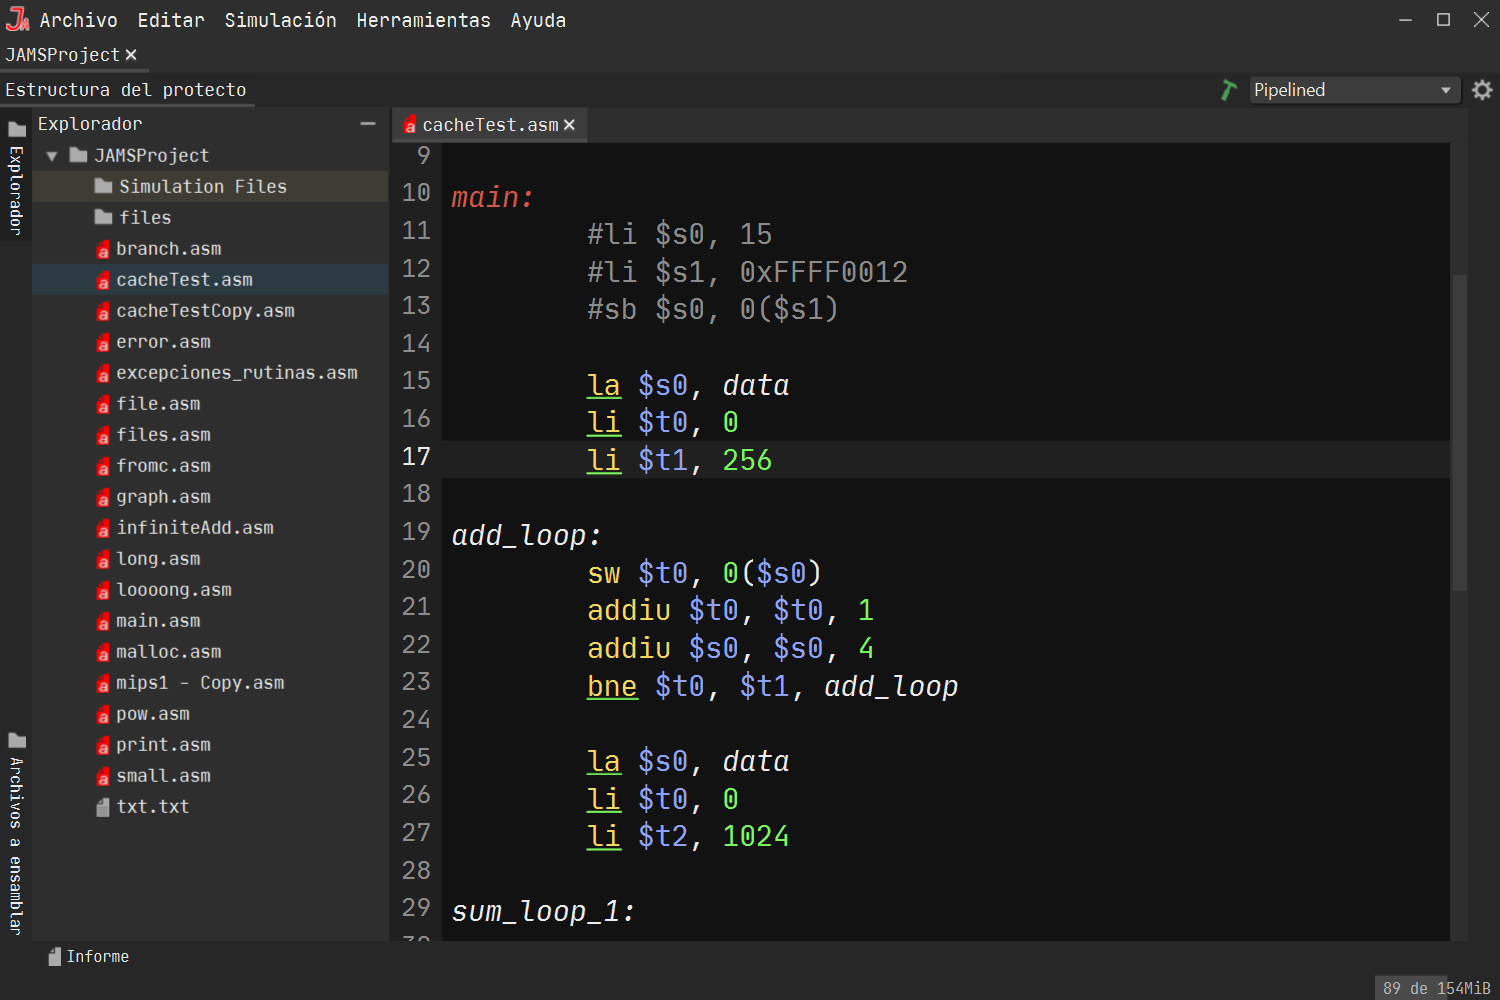
\includegraphics[width=0.8\textwidth]{images/base/jams-text-editor}
    \caption{Editor de texto con estilos inyectados}
    \label{fig:jams-editor-texto}
\end{figure}

\subsection{Referencias entre modelos}\label{subsec:referencias-entre-modelos}

Un modelo puede tener \textbf{referencias a elementos
presentes en otros modelos}.
Este es el caso de las etiquetas y macros globales.
La clase $ProjectGlobalIndex$ permite la
comunicación entre modelos, actuando de intermediador.
Solo los elementos que están dentro de los archivos
de la lista de archivos a ensamblar serán tomados en cuenta.
Para evitar interbloqueos, todas las modificaciones
realizadas en un proyecto son gestionadas en el
mismo hilo.

\subsection{Implementaciones}\label{subsec:implementaciones}

\textit{JAMS} incorpora implementaciones básicas de los
diferentes componentes usados en el editor.
Una de las implementaciones más importantes es la que está
definida en la clase $EditorLineIndex$, la cual
implementa un modelo donde cada línea representa una
unidad autocontenida.

\noindent Otras implementaciones serían la de elementos
básicos y comunes en diferentes lenguajes ensamblador:
las etiquetas, las macros, las llamadas a macros o
los comentarios son ejemplos de elementos ya definidos.

\subsection{Autocompletación}\label{subsec:autocompletacion}

\textit{JAMS} aprovecha los datos proporcionados por
el modelo para implementar una interfaz de autocompletación
que el usuario puede usar en el editor.

\begin{figure}[H]
    \centering
    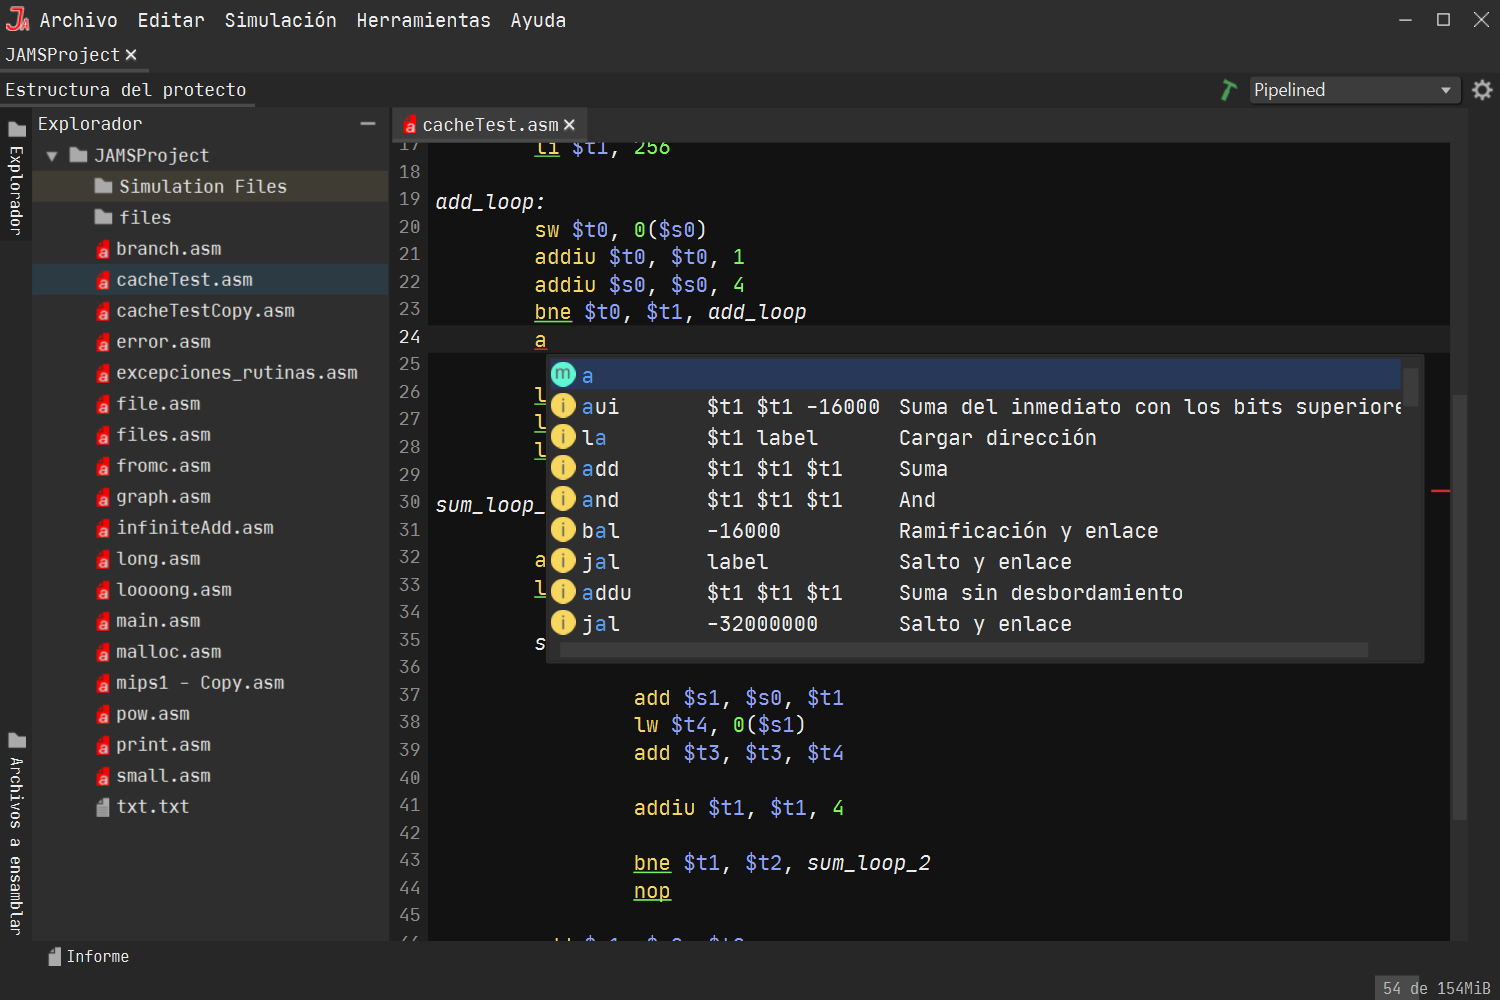
\includegraphics[width=0.8\textwidth]{images/base/jams-autocompletion}
    \caption{Autocompletador del editor de texto}
    \label{fig:jams-autocompletador}
\end{figure}

\noindent Igual que el propio editor de texto, esta interfaz
presenta una estructura modelo-vista-controlador:

\begin{itemize}
    \item \textbf{Controlador:} implementado en dos partes.
    \textit{JAMS} implementa las acciones de la interfaz,
    mientras que el desarrollador debe implementar el
    generador del modelo.
    \item \textbf{Modelo:} contiene los candidatos de
    la interfaz.
    \item \textbf{Vista:} implementa la interfaz que
    muestra los candidatos del modelo.
    \textit{JAMS} implementa una vista por defecto,
    pero los desarrolladores pueden implementar una
    vista propia.
\end{itemize}

\subsection{Documentación}\label{subsec:documentacion}

Como característica final, el editor de texto presenta
una interfaz de documentación que los proyectos
pueden utilizar para documentar sus diferentes
elementos.
Se puede acceder a la documentación con la secuencia por defecto
\textbf{Ctrl + Q}.

\begin{figure}[H]
    \centering
    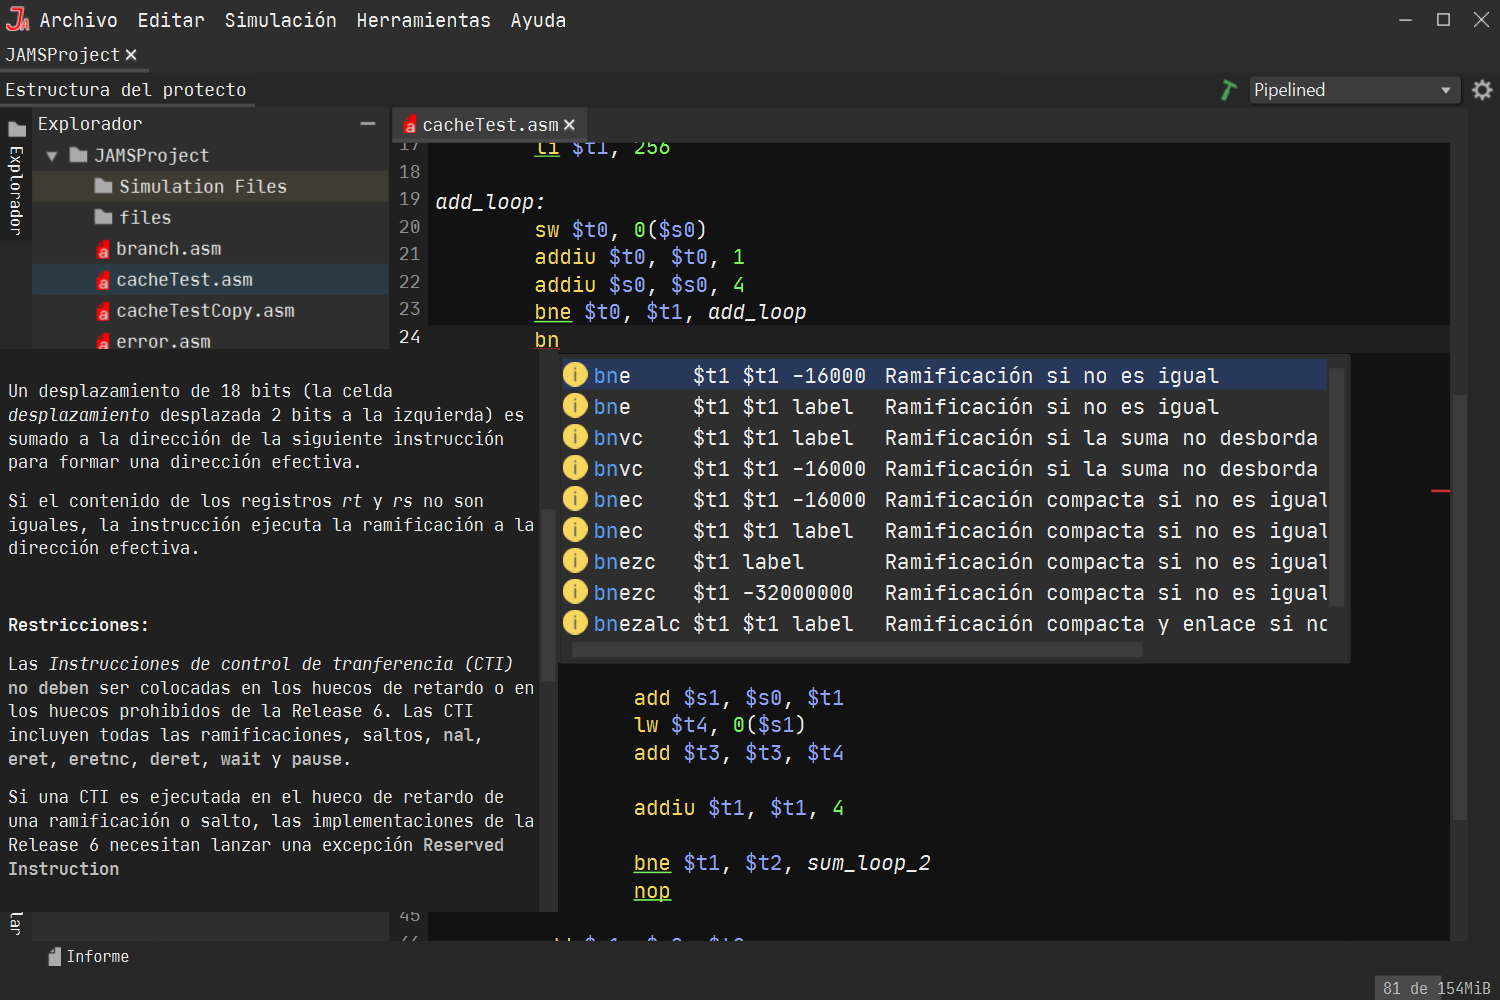
\includegraphics[width=0.8\textwidth]{images/base/jams-documentation}
    \caption{Documentación en el editor de texto}
    \label{fig:jams-documentacion}
\end{figure}
    \chapter{Entorno de desarrollo \textit{MIPS32}}\label{ch:entorno-de-desarrollo-mips32}

El desarrollo de \textit{JAMS} está dividido en dos secciones:
la aplicación base y el entorno de desarrollo \textit{MIPS32}.
\textit{JAMS} da soporte al lenguaje ensamblador \textit{MIPS32}
creando una \textbf{capa sobre la aplicación base},
aprovechando todas las herramientas y características explicadas anteriormente.
En este capítulo se abordarán las capacidades de este entorno,
documentando el ensamblador, el simulador y el editor junto
con sus componentes esenciales.


\section{Ensamblador \textit{MIPS32}}\label{sec:ensamblador-mips32}

El ensamblador \textit{MIP32} de \textit{JAMS} es un ensamblador avanzado
usado para ensamblar proyectos \textit{MIPS32}.
Este ensamblador soporta características avanzadas empleadas
comúnmente al programar en ensamblador, como las macros,
las etiquetas globales o las referencias relativas.

\noindent El ensamblador ensambla el código de un proyecto en cuatro pasos:
descubrimiento, expansión, asignación de direcciones y asignación de valores.
Se utilizará el siguiente programa para comentar los
diferentes pasos del ensamblador:

\begin{lstlisting}[frame=single,label={lst:example.asm}]
    .macro print ( %string )
    .data
text:   .asciiz %string
    .text
    la $a0, text
    li $v0, 4
    syscall
    .endmacro

    .macro printJams ()
    print ("Welcome to JAMS!\n")
    .endmacro

    .text
    .globl main print
main:
local:
    printJams ()
\end{lstlisting}

\subsection{Descubrimiento}\label{subsec:descubrimiento}

En este paso el texto del proyecto se \textbf{descompone en sus primitivas},
permitiendo al ensamblador entender los diferentes componentes de cada línea.
Al final de este paso, las etiquetas globales y las etiquetas de archivo
(etiquetas no definidas dentro de una macro) \textbf{son registradas sin
ningún valor asignado}.

\noindent Las macros de cada archivo también son registradas.
El identificador de una macro es definido por su nombre concatenado
al número de parámetros que necesitan.
Este procedimiento se realiza para dar soporte a la sobrecarga de macros.
En el caso de la macro \textbf{print}, su identificador sería \textbf{print-1}.

\begin{lstlisting}[frame=single,label={lst:descubrimiento}]
Etiquetas globales:
main - XXXXXXXX

Etiquetas del archivo:
local - XXXXXXXX

Macros globales:
print-1

Macros del archivo:
printJams-0
\end{lstlisting}

\subsection{Expansión}\label{subsec:expansion}

En este paso, las llamadas a macros son invocadas,
insertando el código de la macro en la posición de la llamada.
Este código efectúa el primer paso del ensamblador mientras es añadido.
Al ser insertado justo después de la llamada, el código de la macro
también será expandido.

\begin{lstlisting}[frame=single,label={lst:expansion}]
main:
local:
    # Macro printJams-0
    # Macro print-1
    .data # Data returns the previous address.
text:   .asciiz "Welcome to JAMS!\n"
    .text
    la $s0, text
    li $v0, 4
    syscall
    # Endmacro print-1
    # Endmacro printJams-0
\end{lstlisting}

\subsubsection{Alcance}\label{subsubsec:alcance}

Las etiquetas y macros que están dentro de una macro
\textbf{tienen un alcance diferente al del archivo}.
Si la macro es global, el alcance es considerado hijo del alcance global
y no podrá acceder a las etiquetas del archivo que lo invoca.
Si la macro es local, el alcance es considerado hijo del alcance del archivo.

\noindent Cuando un alcance es hijo de otro alcance,
\textbf{el hijo podrá acceder a las etiquetas y macros de su padre}.
El hijo también podrá definir nuevas etiquetas y macros con el mismo
identificador que una etiqueta o macro de su padre.
Aunque este comportamiento está permitido, \textbf{el hijo solo podrá acceder
al elemento que él define}.
Esta funcionalidad es llamada \textbf{ocultamiento o \textit{shadowing}}.

\subsection{Assignación de direcciones}\label{subsec:assignacion-de-direcciones}

Una vez el ensamblador haya expandido las macros,
se asignan las direcciones de todas las instrucciones,
etiquetas y directivas que requieran dirección.
Estas direcciones se asignan de manera secuencial.
Existen directivas que pueden modificar el flujo de la asignación,
como es el caso de la directiva \textbf{.text}.

\begin{lstlisting}[frame=single,label={lst:address-assignation}]
main:
local:
                    # Macro printJams-0
                    # Macro print-1

0x00400000          .data # Data returns the previous address.
0x10010000      text:    .asciiz "Welcome to JAMS!\n"
0x10010010          .text

                    # la is a pseudo-instruction and
                    # it will be split in two instructions
0x00400000          la $s0, text
0x00400008          li $v0, 4
0x0040000c          syscall

                    # Endmacro print-1
                    # Endmacro printJams-0
\end{lstlisting}

\subsection{Asignación de valores}\label{subsec:asignacion-de-valores}

Como paso final, el ensamblador insertará en memoria los valores
que representan las directivas e instrucciones.

\begin{lstlisting}[frame=single,label={lst:value-assignation}]
                    # Macro printJams-0
                    # Macro print-1

0x10010000          Welcome to JAMS!\n\0
0x00400000          0x3c011001 # la $a0, text
0x00400004          0x34240000
0x00400008          0x24020004 # li $v0, 4
0x0040000c          0x0000000c # syscall

                    # Endmacro print-1
                    # Endmacro printJams-0
\end{lstlisting}

\subsection{Características avanzadas}\label{subsec:características-avanzadas}

El ensamblador permite el uso de técnicas avanzadas en
el desarrollo de aplicaciones en lenguaje ensamblador.

\subsubsection{Referencias relativas}\label{subsubsec:referencias-relativas}

Una directiva o instrucción puede \textbf{referenciar a una etiqueta de manera
relativa} con las referencias especiales \textbf{+} y \textbf{-}.
La referencia \textbf{+} hace referencia a la etiqueta siguiente.
La referencia \textbf{-} hace referencia a la etiqueta anterior.
Las referencias relativas \textbf{solo pueden hacer referencia
a etiquetas del mismo alcance}.
No pueden hacer referencia a etiquetas de un alcance mayor.

\begin{lstlisting}[frame=single,label={lst:relative-reference}]
main:
    li $s0, 0
    li $s1, 10
loop:
    printJams ()
    addi $s0, $s0, 1
    bne $s0, $s1, -
\end{lstlisting}

\subsubsection{Macros anidadas}\label{subsubsec:macros-anidadas}

Una macro puede ser definida dentro de otra macro.
Esto es conocido como una \textbf{macro anidada}.
Esta macro solo podrá ser accedida en el alcance de la macro
en la que está declarada.

\begin{lstlisting}[frame=single,label={lst:nested-macro}]
    .macro printJams ()
    .macro print (%string)
    .data
text:   .asciiz %string
    .text
    la $a0, text
    li $v0, 4
    syscall

    .endmacro
    print ("Welcome to JAMS!\n")
    .endmacro
\end{lstlisting}

\section{Instrucciones}\label{sec:instrucciones}

Las instrucciones son la parte más importante de un lenguaje ensamblador.
JAMS permite crear y gestionar instrucciones de una manera modular.

\subsection{Estructura de una instrucción}\label{subsec:estructura-de-una-instruccion}

Todas las instrucciones implementan la interfaz \textbf{Instruction}.
Esta interfaz define conceptos básicos de una instrucción,
como su nombre, su mnemónico, su documentación o sus parámetros.
Esta interfaz también define los métodos \textbf{match},
usada para comprobar si un mnemónico y un conjunto de parámetros
representan una instrucción.
Estos métodos son utilizados por el ensamblador y el editor para saber qué
instrucción define una línea.
Por último, la interfaz define el método \textit{assemble}, el
cual traduce la instrucción en un conjunto de instrucciones ensambladas.
Este método debe ser implementado por las clases hijas.
Esta interfaz es implementada por dos clases abstractas básicas:
\textbf{BasicInstruction} y \textbf{PseudoInstruction}.

\subsection{Instrucciones básicas}\label{subsec:instrucciones-basicas}

Las instrucciones básicas (representadas por la clase abstracta
\textbf{BasicInstruction}) representan instrucciones normales del ensamblador.
Estas instrucciones tienen una traducción directa a código máquina.
Esta clase abstracta define elementos más concretos, como el código de operación,
la unidad aritmético-lógica donde la instrucción debe ejecutarse y
un nuevo método \textbf{match} que permite saber si un código de instrucción
representa la instrucción.
Esta clase define los métodos abstractos \textbf{assembleBasic}
y \textbf{assembleFromCode}.
Estos métodos permiten crear un elemento de tipo \textbf{AssembledInstruction}
mediante un código de instrucción o un conjunto de parámetros.
El método \textbf{assemble} de la interfaz \textbf{Instruction}
está implementada por esta clase.

\noindent Todas las instrucciones básicas requieren dos
constantes globales en su implementación:
\begin{itemize}
    \item \textbf{MNEMONIC:} es un \textbf{String} que define
    el mnemónico de la instrucción.
    \item \textbf{PARAMETER\_TYPES:} es un elemento de tipo
    \textbf{InstructionParameterTypes} que representa
    los tipos de los parámetros de la instrucción.
\end{itemize}

\begin{lstlisting}[language=Java,style=java,frame=single,label={lst:basic-instruction}]
public class InstructionAbsDouble extends
    BasicRFPUInstruction<InstructionAbsDouble.Assembled> {

    public static final String MNEMONIC = "abs.d";
    public static final InstructionParameterTypes PARAMETER_TYPES =
        new InstructionParameterTypes(
            ParameterType.EVEN_FLOAT_REGISTER,
            ParameterType.EVEN_FLOAT_REGISTER
        );
}
\end{lstlisting}

\subsection{Pseudo-instrucciones}\label{subsec:pseudo-instrucciones}

Las pseudo-instrucciones son instrucciones que el ensamblador
convertirá en un conjunto de instrucciones básicas.
Pueden considerarse un conjunto de instrucciones que ejecutan una acción común.
Estas instrucciones están representadas por la clase
\textbf{PseudoInstruction},
la cual define el método \textbf{getInstructionAmount}.
Este método le permite saber al ensamblador cuántas instrucciones
debe esperar que la pseudo-instrucción dé como resultado dependiendo
del conjunto de parámetros dado.
La clase también implementa varios métodos estáticos que sirven
de utilidad para implementar pseudo-instrucciones rápidamente.

\noindent Como ejemplo, la implementación de la pseudo-instrucción
\textbf{addi} sería la siguiente:

\begin{lstlisting}[language=Java,style=java,frame=single,label={lst:pseudo-instruction}]
public class PseudoInstructionAddi extends PseudoInstruction {

    public static final String MNEMONIC = "addi";

    public static final InstructionParameterTypes PARAMETER_TYPES =
        new InstructionParameterTypes(
            ParameterType.REGISTER,
            ParameterType.REGISTER,
            ParameterType.SIGNED_16_BIT
        );

    public PseudoInstructionAddi() {
        super(MNEMONIC, PARAMETER_TYPES);
    }

    @Override
    public int getInstructionAmount(String[] parameters) {
        return 2;
    }

    @Override
    public AssembledInstruction[] assemble(
            InstructionSet set,
            int address,
            ParameterParseResult[] parameters
    ) {
        var instructions = instructions(set,
                InstructionAddiu.class, InstructionAdd.class);

        var addiu = parameters(AT, ZERO, parameters[2]);
        var add = parameters(parameters[0], AT, parameters[1]);

        return assemble(instructions, addiu, add);
    }
}
\end{lstlisting}

\subsection{Instrucciones ensambladas}\label{subsec:instrucciones-ensambladas}

La clase \textbf{AssembledInstruction} representa una instrucción ensamblada.
Esta clase guarda el entero que representa el código de instrucción,
la instrucción que ha creado la instrucción ensamblada
(puede ser una instrucción básica o una pseudo-instrucción),
y la instrucción básica que representa.
Este tipo de elementos sirve únicamente para guardar
la información sobre la instrucción.
Las clases hijas de \textbf{AssembledInstruction} pueden definir métodos útiles
que permitan extraer parámetros del código de instrucción.

\subsection{Ejecución de una instrucción}\label{subsec:ejecución-de-una-instruccion}

Por último, las instrucciones también están definidas por una clase
\textbf{InstructionExecution}.
Esta clase implementa la ejecución de una instrucción en una arquitectura,
e implementa muchos métodos útiles que los hijos pueden usar para definir
la ejecución de sus instrucciones.
La clase \textbf{InstructionExecution} no debe ser extendida directamente,
si no que se debe extender la clase \textbf{SingleCycleExecution}
para ejecuciones uni-ciclo y \textbf{MultiCycleExecution} para ejecuciones
multi-ciclo o segmentadas.
Estas ejecuciones deben ser registradas en la instrucción
empleando el método \textbf{addExecutionBuilder}.

\subsection{Conjuntos de instrucciones}\label{subsec:conjuntos-de-instrucciones}

Las instrucciones están agrupadas en conjuntos de instrucciones.
Un proyecto utilizará un conjunto de instrucciones para ensamblar su código,
ayudar al usuario en el editor e interpretar el código máquina del simulador.
Los conjuntos de instrucciones están gestionados por el gestor
\textbf{InstructionSetManager}.
    \chapter{Herramientas}\label{ch:herramientas}

En este capítulo se abordarán las diferentes herramientas,
tanto generales como específicas para el entorno \textit{MIPS32},
presentes en \textit{JAMS}.


\section{Explorador}\label{sec:explorador}

El explorador es la \textbf{herramienta más importante de todo el editor}.
Permite \textbf{visualizar las carpetas y archivos del proyecto}
de una manera rápida y sencilla.
El explorador es una herramienta pensada para que cualquier tipo de proyecto
pueda implementar su version de una manera rápida y sencilla.
La tecnología detrás del explorador se \textbf{usa en diferentes partes de la aplicación},
como pueden ser la sección de acciones y las herramientas de etiquetas y archivos
a ensamblar.

\begin{figure}[H]
    \centering
    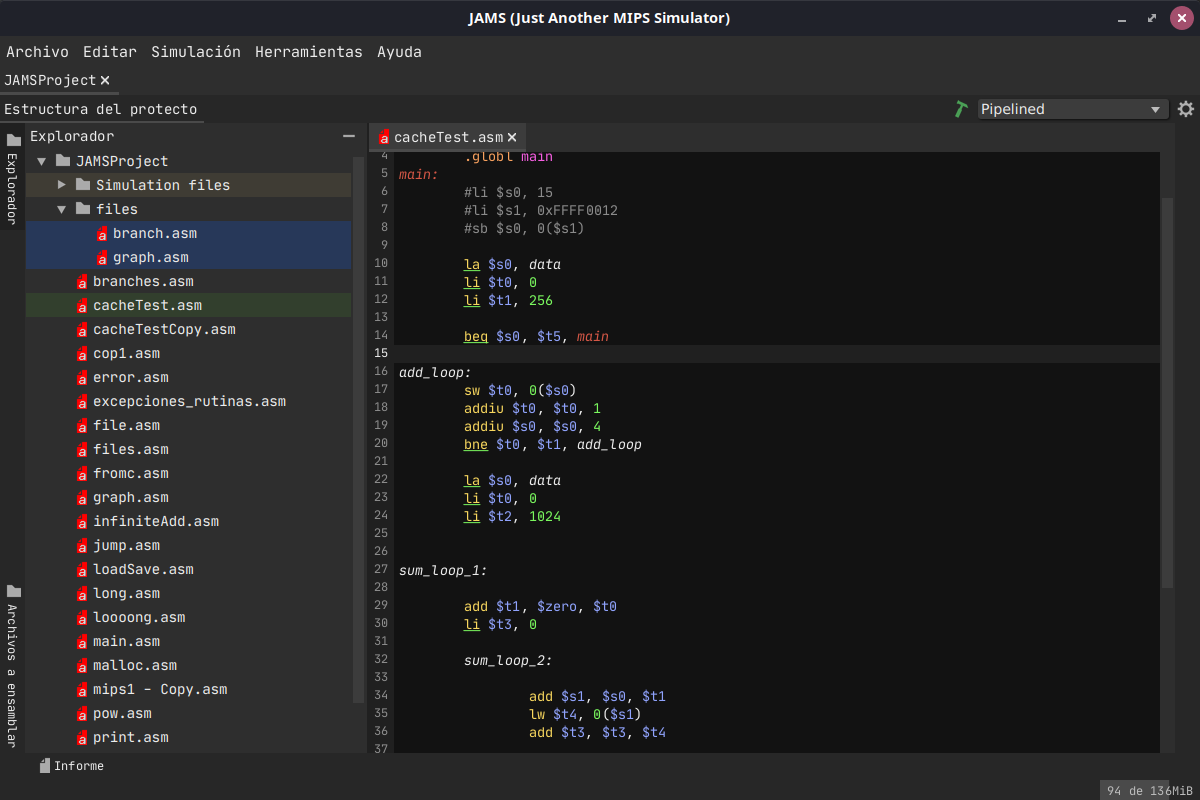
\includegraphics[width=0.8\textwidth]{images/tools/jams-explorer}
    \caption{Explorador}
    \label{fig:jams-explorer}
\end{figure}

\noindent El explorador presenta las siguientes funcionalidades:
\begin{itemize}
    \item \textbf{Abrir archivos:} la principal funcionalidad del editor
    es poder abrir archivos en el editor.
    Haciendo doble clic en un archivo o seleccionándolo y pulsando
    $enter$, se mostrará un editor especializado para el archivo
    en cuestión.
    \item \textbf{Desplazamiento:} el usuario puede desplazarse por el
    explorador utilizando las flechas del teclado.
    El usuario también puede ir seleccionando archivos mientras se
    mueve manteniendo pulsado la tecla $shift$.
    \item \textbf{Selección:} el usuario también puede seleccionar
    elementos del explorador de manera selectiva manteniendo
    pulsada la tecla $ctrl$ mientras se emplea el botón principal
    del ratón en los elementos a seleccionar.
    \item \textbf{Menú de contexto:} el menú de contexto muestra
    una lista de acciones aplicables a la selección.
    El usuario podrá desplegar este menu usando el botón secundario
    del ratón.
\end{itemize}

\noindent El explorador de archivos es un explorador específico
que le permite al usuario visualizar la estructura del proyecto
actual.
Este explorador mostrará sus elementos con un fondo diferente en
casos especiales:
\begin{itemize}
    \item \textbf{Azul:} el elemento está seleccionado.
    \item \textbf{Verde:} el elemento está dentro de la lista de
    archivos a ensamblar.
    \item \textbf{Verde azulado}: el elemento está seleccionado y
    dentro de la lista de archivos a ensamblar.
    \item \textbf{Marrón:} el elemento no es considerado
    parte del proyecto.
\end{itemize}


\section{Archivos a ensamblar:}\label{sec:archivos-a-ensamblar:}

La herramienta de archivos a ensamblar permite
ver, ordenar, eliminar y modificar los \textbf{archivos que se van a ensamblar}.

\begin{figure}[H]
    \centering
    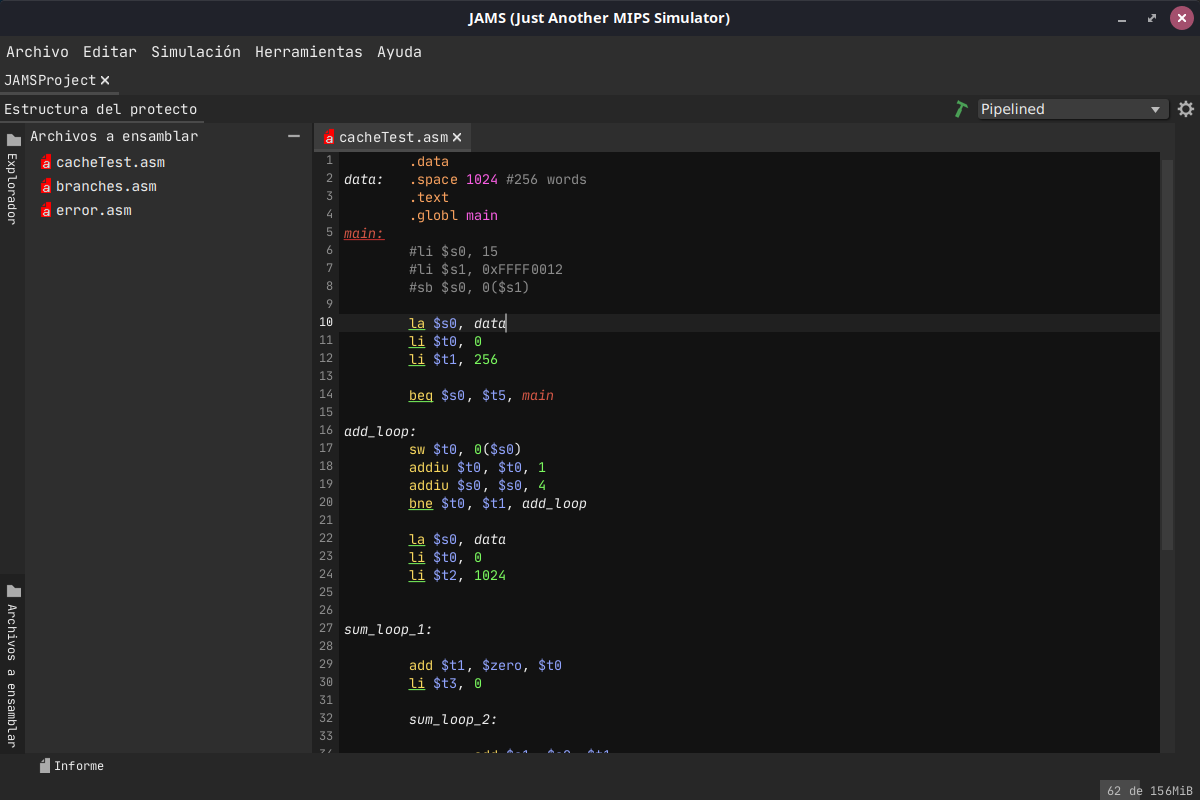
\includegraphics[width=0.8\textwidth]{images/tools/jams-files-to-assemble}
    \caption{Archivos a ensamblar}
    \label{fig:jams-files-to-assemble}
\end{figure}

\noindent Pueden haber tipos de proyecto donde el
orden de los archivos a ensamblar importe.
Esta herramienta permite al usuario \textbf{ordenar los archivos}
a ensamblar \textbf{arrastrándolos a la posición deseada}.
La herramienta también permite \textbf{eliminar un archivo} de la lista
mediante un menú de contexto que el usuario puede abrir usando
el botón secundario del ratón en el archivo a eliminar.


\section{Informe}\label{sec:informe}

La herramienta \textbf{informe} te permite \textbf{visualizar el resultado}
de los ensamblajes que hagas en tu proyecto.
También le permite a otras herramientas informar sobre cambios de estados y errores.

\begin{figure}[H]
    \centering
    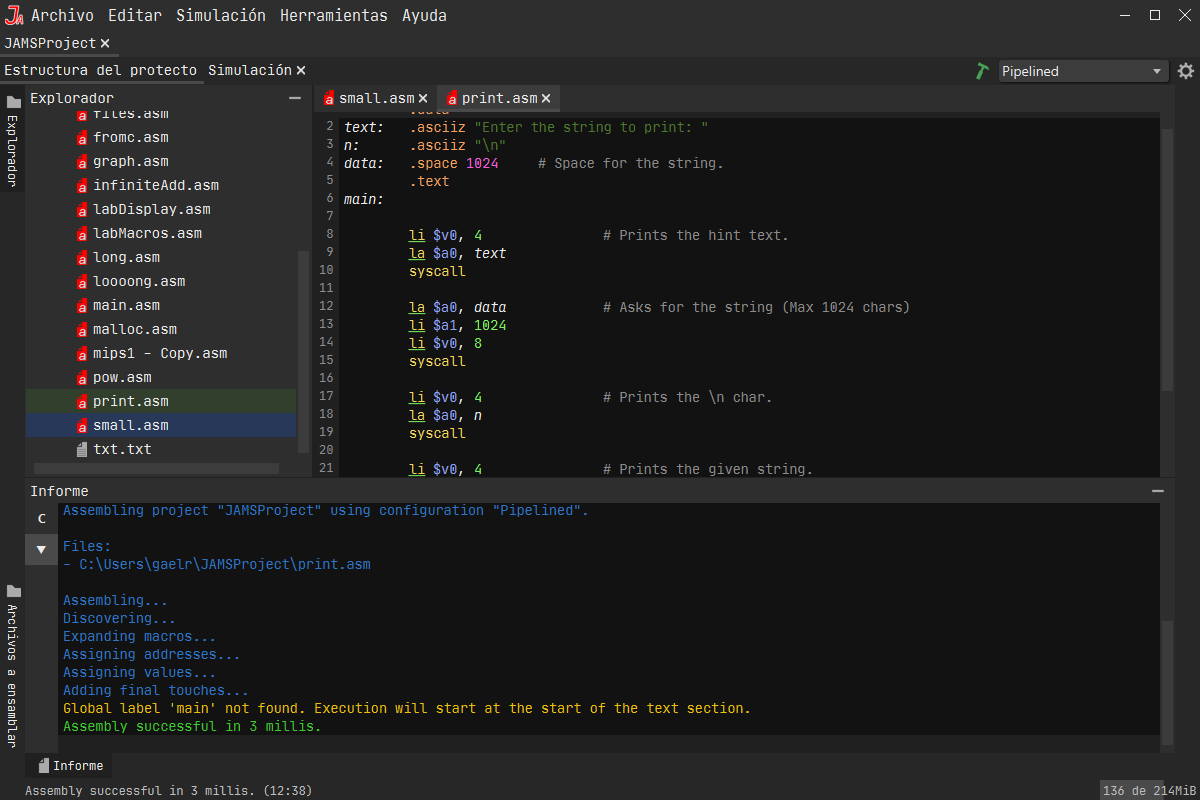
\includegraphics[width=0.8\textwidth]{images/tools/jams-log}
    \caption{Informe}
    \label{fig:jams-log}
\end{figure}

\noindent El informe contiene dos botones con el que se puede interactuar:
\begin{itemize}
    \item El botón $C$ permite limpar el informe, eliminando todo el
    texto presente en él.
    \item El botón $\nabla$ permite habilitar o deshabilitar el desplazamiento
    automático al final del visualizador.
    Si esta opción está habilitada, el visualizador se desplazará
    automáticamente hasta el final del visualizador cuando un
    nuevo mensaje entra en él.
\end{itemize}


\section{Memoria}\label{sec:memoria-herramienta}

La herramienta \textbf{memoria} permite visualizar la información que
contiene la memoria y las cachés de un simulador en el estado actual.
Esta herramienta muestra la memoria en celdas de 4 bytes,
lo cual permite una visualización óptima para arquitecturas
basadas en 32 bits.

\begin{figure}[H]
    \centering
    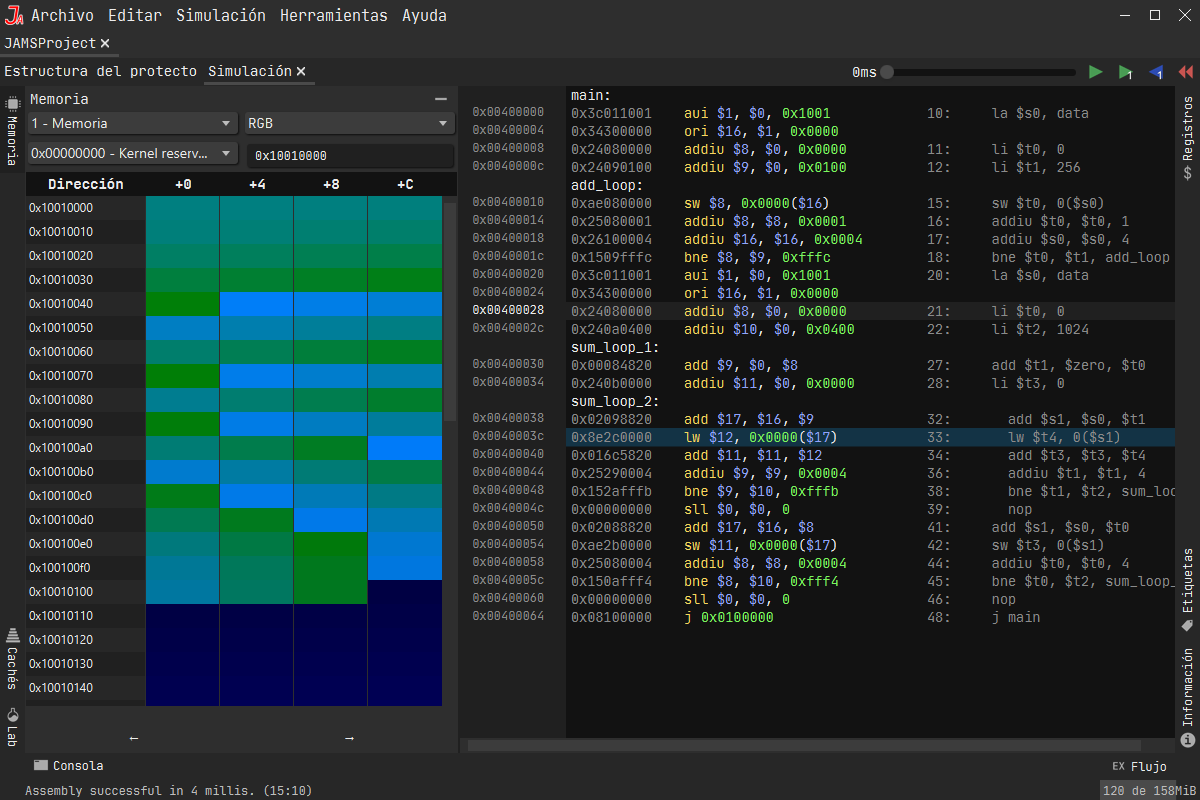
\includegraphics[width=0.8\textwidth]{images/tools/jams-memory}
    \caption{Herramienta de memoria}
    \label{fig:jams-memory}
\end{figure}

\noindent El primer desplegable de la herramienta permite elegir qué
memoria se desea visualizar.
La lista de memorias está ordenada por nivel, siendo la primera
memoria la caché de nivel 1.
Si la simulación no contiene ninguna caché,
este desplegable solo mostrará la memoria principal.

\noindent El segundo desplegable contiene diferentes opciones
en las que los datos de la memoria se puede visualizar.
Las opciones disponibles son las siguientes:

\begin{itemize}
    \item \textbf{Binario:} muestra cada valor en binario.
    \item \textbf{Caracteres:} muestra cada valor como un conjunto de
    cuatro caracteres ASCII\@.
    \item \textbf{Decimal:} muestra cada valor en decimal.
    Esta es la opción por defecto.
    \item \textbf{Coma flotante de precisión doble:}  muestra cada valor
    en coma flotante de doble precisión.
    La parte más representativa es el valor de la siguiente celda de memoria.
    \item \textbf{Texto inglés:} muestra cada valor como un texto en inglés.
    \item \textbf{Coma flotante de precisión simple:} muestra cada
    valor en coma flotante.
    \item \textbf{Hexadecimal:} muestra cada valor en hexadecimal.
    \item \textbf{Entero de 64 bits:} muestra cada valor como un número de 64 bits.
    La parte más representativa es el valor de la siguiente celda de memoria.
    \item \textbf{Octal:} muestra cada valor en octal.
    \item \textbf{RGB:} muestra cada valor como un color RGB\@.
    El cuarto más representativo del valor queda en desuso.
    \item \textbf{RGBA:} muestra cada valor como un color RGBA\@.
    \item \textbf{Romano:} muestra cada valor como un número romano.
\end{itemize}

\noindent El usuario puede desplazarse a través de la herramienta
de diferentes maneras: \textbf{seleccionando una sección}
en el tercer desplegable, \textbf{insertando una dirección}
o \textbf{usando las flechas de movimiento}.
Una vez identificado la celda deseada, el usuario podrá
\textbf{modificar su valor} haciendo doble clic en ella.
El nuevo value puede estar representado en binario, octal,
decimal o hexadecimal.


\section{Herramienta de cachés}\label{sec:herramienta-de-caches}

La herramienta \textbf{cachés} muestra información
sobre las cachés del simulador.
La herramienta está conformada por dos secciones:
las estadísticas y el registro.
En las estadísticas se muestran las operaciones,
aciertos y fallos de una caché, mientras que en el
registro se muestran todas las acciones que una
caché ha realizado junto con su resultado.

\begin{figure}[H]
    \centering
    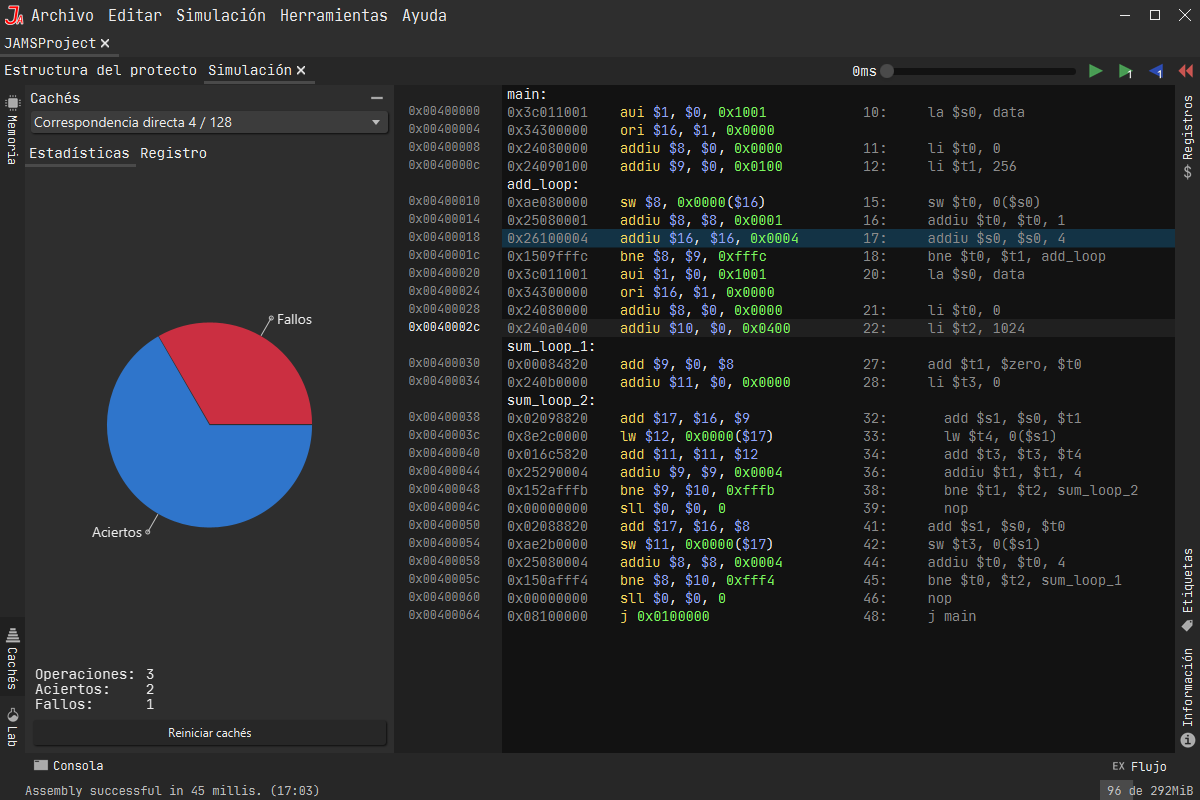
\includegraphics[width=0.8\textwidth]{images/tools/jams-caches}
    \caption{Herramienta de cachés}
    \label{fig:jams-caches-stats}
\end{figure}

\noindent A diferencia de otras herramientas, el registro no se
borra cuando se reinicia la simulación o se deshace un paso.
La herramienta está diseñada así para poder visualizar fácilmente los cambios de la caché.

\begin{figure}[H]
    \centering
    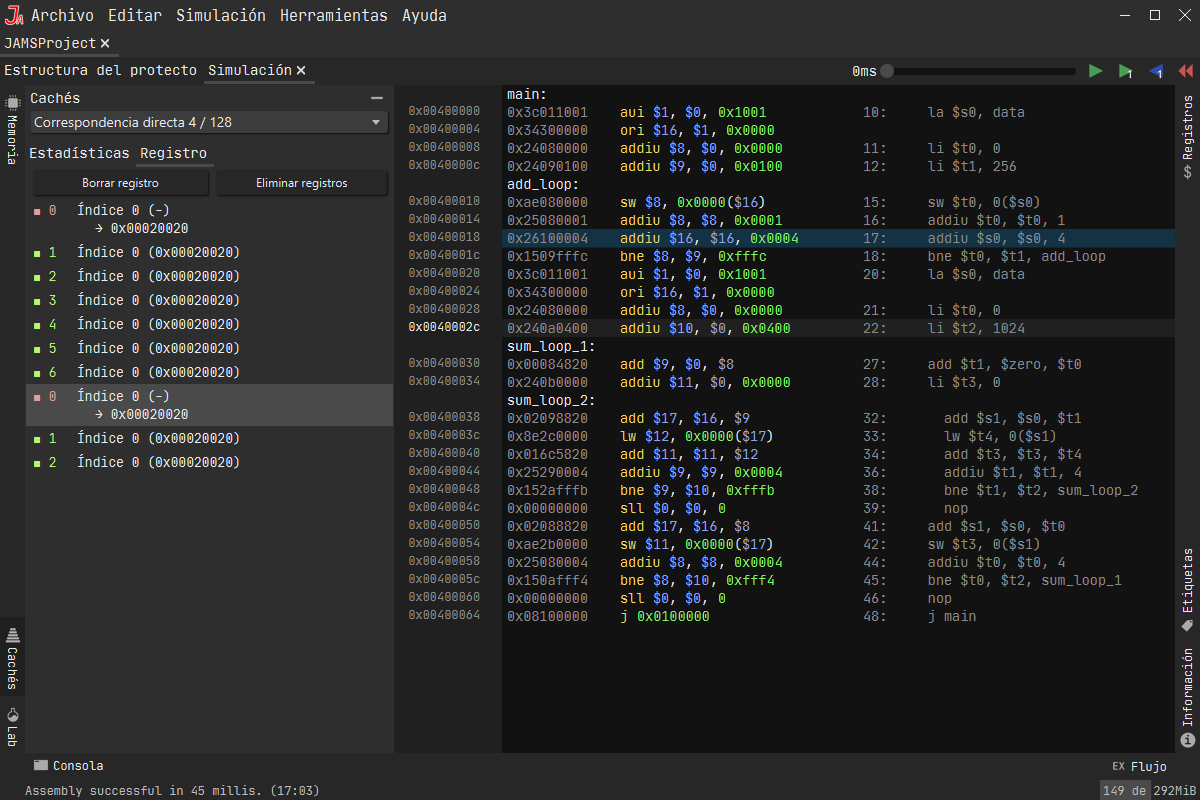
\includegraphics[width=0.8\textwidth]{images/tools/jams-caches-log}
    \caption{Registro de la herramienta de cachés}
    \label{fig:jams-caches-log}
\end{figure}

\section{Laboratorio}\label{sec:laboratorio}

La herramienta \textbf{laboratorio} simula varios componentes básicos
externos conectados a un simulador \textit{MIPS32}.
En concreto, la herramienta simula cuatro componentes básicos:
dos visualizadores de siete segmentos, un teclado hexadecimal,
un generador de interrupciones y un contador.

\begin{figure}[H]
    \centering
    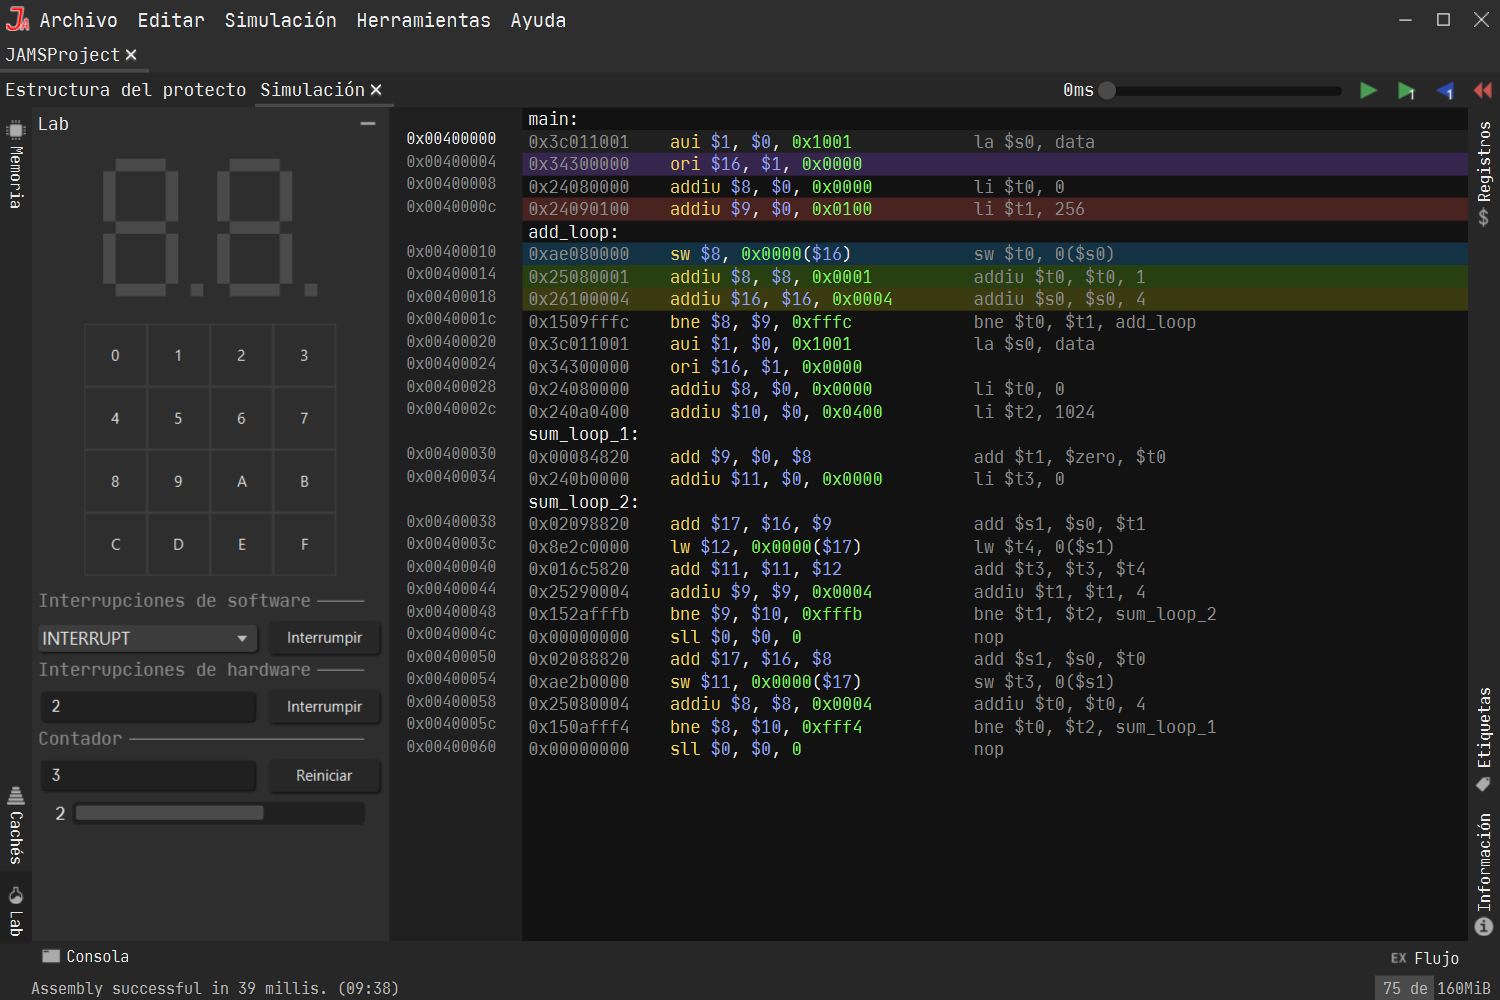
\includegraphics[width=0.8\textwidth]{images/tools/jams-lab}
    \caption{Laboratorio}
    \label{fig:jams-lab}
\end{figure}

\subsection{Visualizador de siete segmentos}\label{subsec:visualizador-de-siete-segmentos}

Un visualizador de siete segmentos \textbf{permite representar un dígito o letra},
y está controlado por el contenido de un \textbf{byte en memoria}.
En concreto, cada segmento del visualizador está controlado por un bit del byte.
Los bits que controlan cada segmento son los siguientes:

\begin{figure}[H]
    \centering
    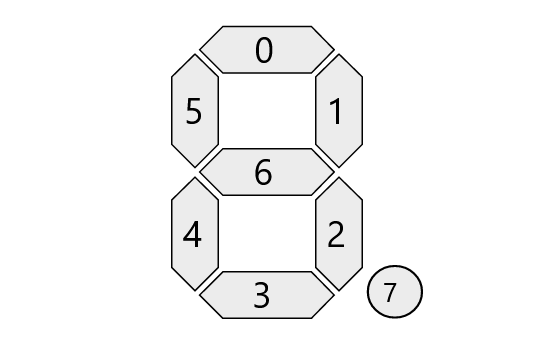
\includegraphics[width=0.5\textwidth]{images/tools/jams-seven-segment}
    \caption{Visualizador de siete segmentos}
    \label{fig:jams-seven-segment}
\end{figure}

\noindent Si, por ejemplo, se desea el dígito $5$ en el visualizador,
se debe guardar en la dirección del byte el valor $0b01101101$.

\begin{figure}[H]
    \centering
    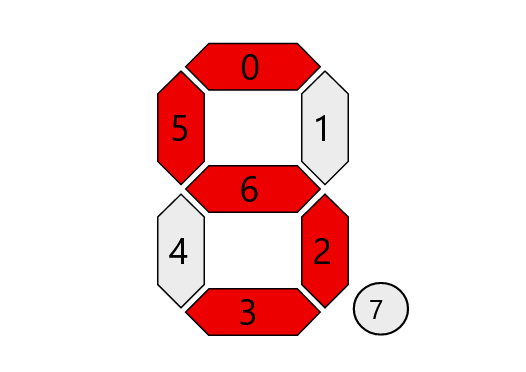
\includegraphics[width=0.5\textwidth]{images/tools/jams-seven-segment-active}
    \caption{Visualizador de siete segmentos representando un 5}
    \label{fig:jams-seven-segment-active}
\end{figure}

\noindent Las \textbf{direcciones de memoria por defecto} que controlan los dos
visualizadores son la dirección $0xffff0010$ para el visualizador derecho y
$0xffff0011$ para el visualizador izquierdo.
Estos valores se pueden cambiar en la configuración,
en el apartado \textbf{Simulación > MIPS}.

\subsection{Teclado hexadecimal}\label{subsec:teclado-hexadecimal}

El segundo componente de la herramienta es el teclado hexadecimal.
Este teclado \textbf{permite introducir valores} que el
simulador puede interpretar.
Cuando el usuario pulsa uno de los botones,
\textit{JAMS} genera una \textbf{interrupción \textit{hardware} de nivel 3}.
El programa puede interpretar el evento implementando un gestor
de excepciones en la dirección por defecto $0x80000260$.

\noindent Para saber qué \textbf{botones del teclado están activados},
se deben leer las direcciones de memoria por defecto $0xffff0013$ y $0xffff0014$.
Cada bit de los dos bytes representan un botón en el teclado.
Si un bit contiene el valor 1, el botón que representa está seleccionado.

\noindent Como ejemplo: si el valor de la dirección de memoria
$0xffff0013$ es $0b00000100$ y el valor de la dirección de memoria
$0xffff0014$ es $0b10000100$, los botones 2, A y F están seleccionados.

\subsection{Generador de interrupciones y contador}\label{subsec:generador-de-interrupciones-contador}

El generador de interrupciones \textbf{permite generar} tanto
interrupciones \textit{software} como interrupciones \textit{hardware}.
En el caso de las interrupciones \textit{software},
la herramienta permite definir la causa de la interrupción.

\noindent El contador es una pequeña herramienta
\textbf{que genera una interrupción \textit{hardware}}
de nivel 2 cada cierto número de ciclos especificados por el usuario.
Este valor se puede asignar desde la interfaz o escribiéndolo
en la dirección de memoria $0xffff0012$.

\section{Consola}\label{sec:consola}

La \textbf{consola permite ver los mensajes} de la aplicación
e introducir valores que el simulador puede interpretar.
La consola \textbf{actúa de intermediador principal}
entre el usuario y la aplicación.

\begin{figure}[H]
    \centering
    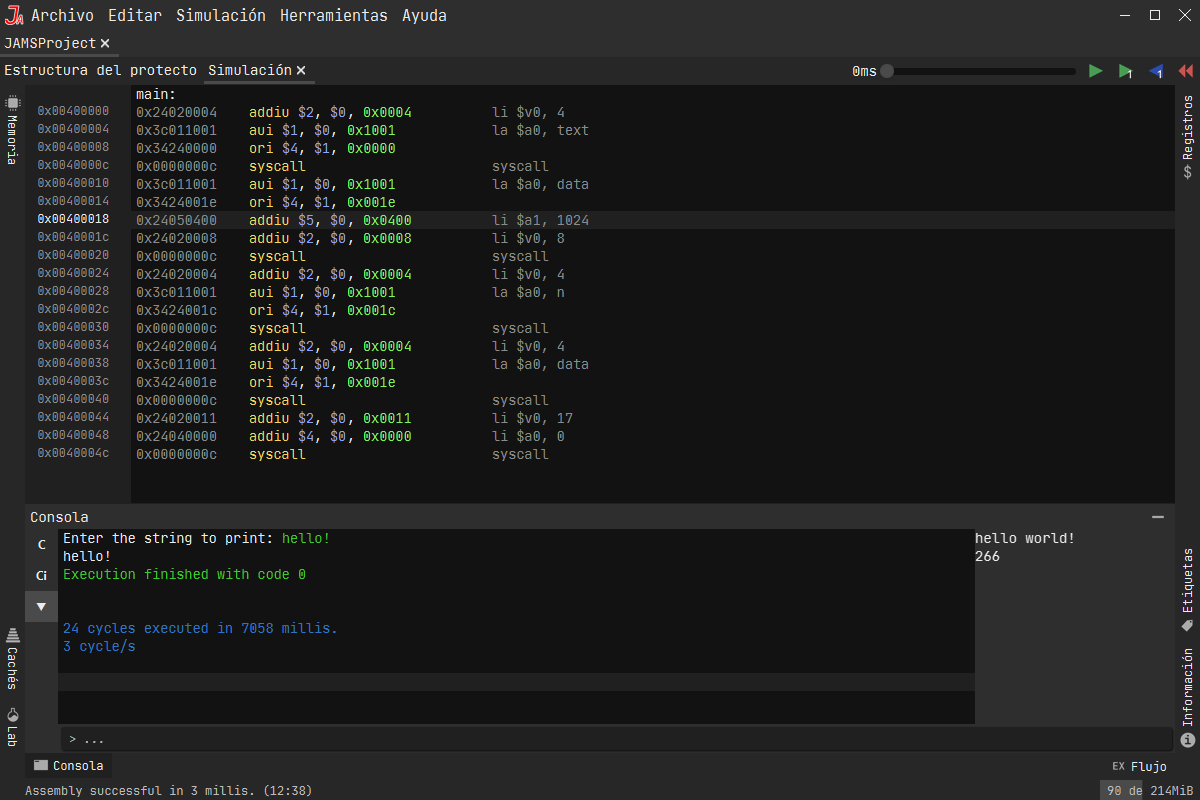
\includegraphics[width=0.8\textwidth]{images/tools/jams-console}
    \caption{Consola}
    \label{fig:jams-console}
\end{figure}

\noindent El visualizador muestra los mensajes que la aplicación
imprime mediante llamadas del sistema.
También muestra el resultado de la ejecución al terminar la simulación.
La consola permite enviar mensajes a la aplicación mediante la barra de
texto de la parte inferior de la herramienta.
Los mensajes \textbf{quedarán guardados} en una cola de mensajes
hasta que la simulación los lea.
El usuario \textbf{puede eliminar mensajes} de la cola
pulsando el mensaje que quiere eliminar.

\noindent La consola contiene tres botones con el que se puede interactuar:
\begin{itemize}
    \item El botón $C$ permite limpar el informe, eliminando todo el
    texto presente en él.
    \item El botón $Ci$ permite limpiar la cola de mensajes.
    \item El botón $\nabla$ permite habilitar o deshabilitar el desplazamiento
    automático al final del visualizador.
    Si esta opción está habilitada, el visualizador se desplazará
    automáticamente hasta el final del visualizador cuando un
    nuevo mensaje entra en él.
\end{itemize}

\section{Herramienta de flujo}\label{sec:herramienta-de-flujo}

La herramienta \textbf{flujo} permite ver el flujo de ejecución del simulador.
La herramienta tiene una funcionalidad puramente visual:
\textbf{no permite editar} ningún aspecto del simulador.
El usuario puede usar la barra deslizadora para cambiar el tamaño de las columnas,
y puede desplazarse de manera sencilla arrastrando el ratón.

\begin{figure}[H]
    \centering
    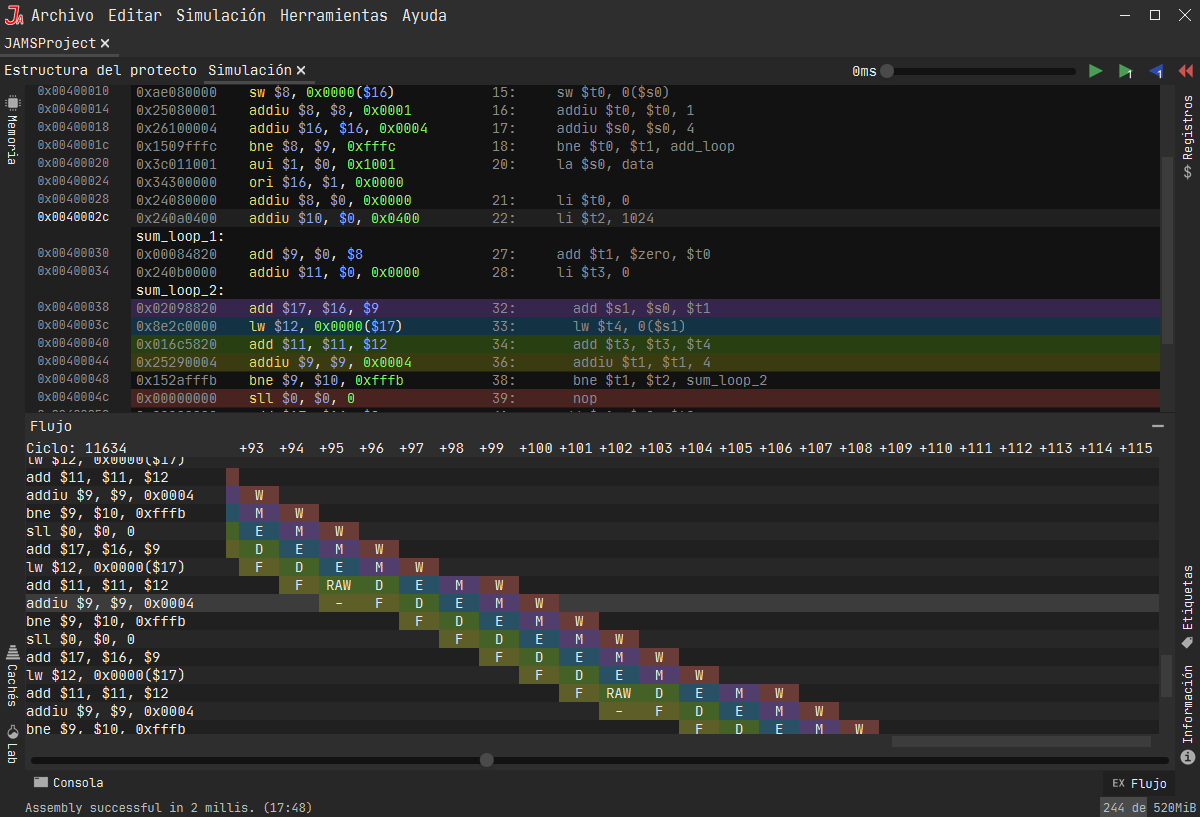
\includegraphics[width=0.8\textwidth]{images/tools/jams-flow}
    \caption{Herramienta de flujo}
    \label{fig:jams-flow}
\end{figure}

\noindent El visualizador únicamente representa un número máximo de instrucciones.
Este número es por defecto $100$, y se puede cambiar en la configuración.
El número de ciclo representado en la parte superior izquierda representa
al \textbf{primer ciclo representado por el visualizador} de flujo.
Cada columna contiene un número que representa su ciclo con respecto al ciclo inicial.

\section{Información}\label{sec:informacion}

La herramienta \textbf{información} es una herramienta muy sencilla
que informa sobre aspectos generales del simulador.

\begin{figure}[H]
    \centering
    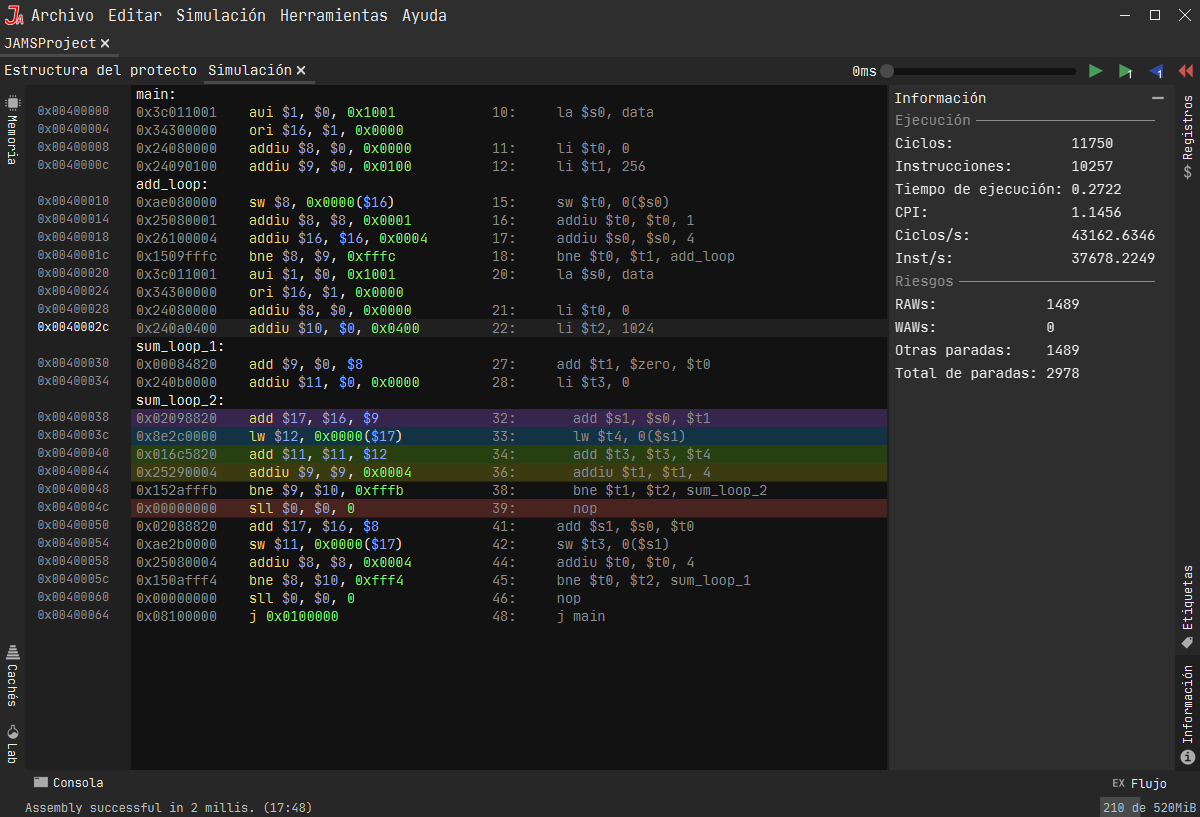
\includegraphics[width=0.8\textwidth]{images/tools/jams-information}
    \caption{Información}
    \label{fig:jams-information}
\end{figure}

\noindent La herramienta muestra los ciclos ejecutados,
instrucciones ejecutadas, tiempo de ejecución, ciclos por instrucción,
ciclos por segundo e instrucciones por segundo de una simulación.
Dependiendo del tipo de arquitectura, la simulación también podrá
\textbf{mostrar otros tipos de datos}, como los riesgos de ejecución.

\section{Herramienta de etiquetas}\label{sec:herramienta-de-etiquetas}

La herramienta \textbf{etiquetas} muestra información sobre las etiquetas
utilizadas por en ensamblador para generar la simulación.

\begin{figure}[H]
    \centering
    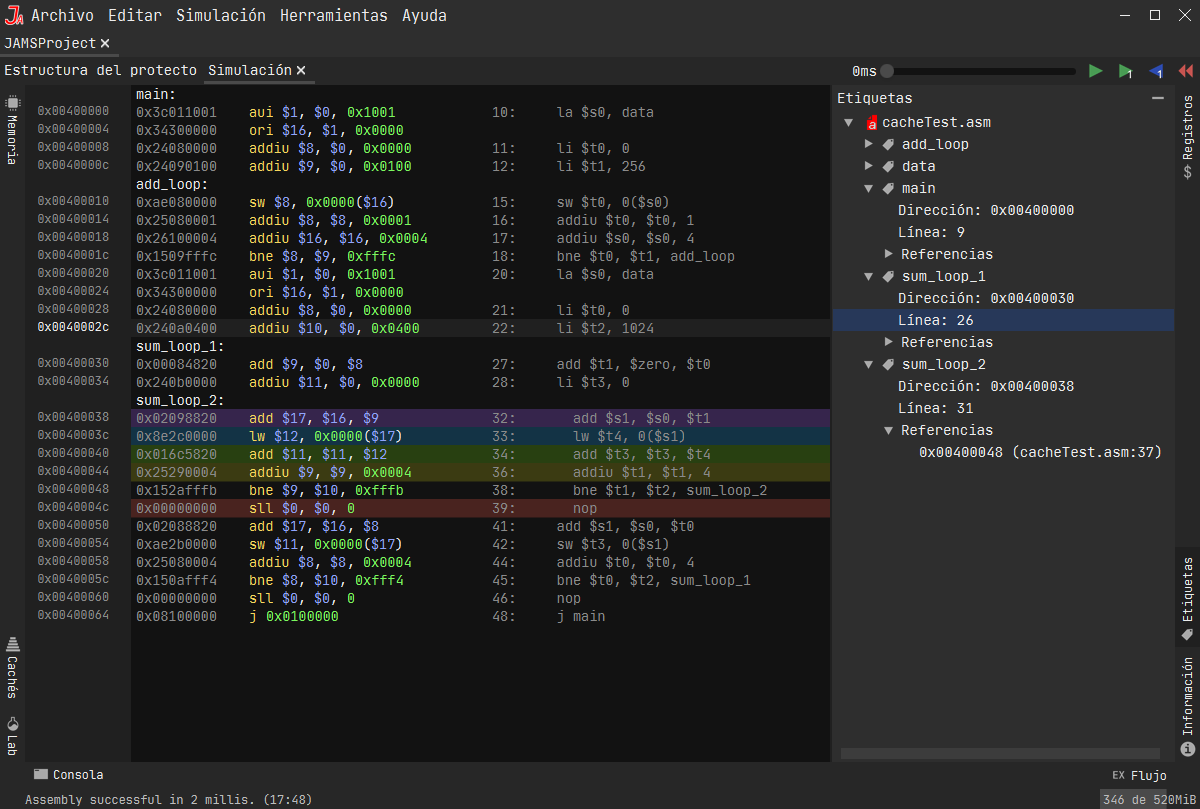
\includegraphics[width=0.8\textwidth]{images/tools/jams-labels}
    \caption{Herramienta de etiquetas}
    \label{fig:jams-labels}
\end{figure}

\noindent Las etiquetas están \textbf{catalogadas por archivos}.
Cada etiqueta contiene su dirección asignada,
la línea en la que fue declarada en el archivo y las referencias.

Cada referencia contiene la dirección en la que fue referenciada,
la línea del archivo y el archivo en sí donde se encuentra dicha referencia.
Pulsando el botón secundario del ratón sobre una etiqueta
o una referencia el usuario puede acceder al \textbf{menú de contexto}
donde se puede visualizar la dirección de memoria en el visualizador
de instrucciones o en la memoria.

\section{Herramienta de registros}\label{sec:herramienta-de-registros}

La herramienta de \textbf{registros} muestra información sobre
los registros de la simulación.

\noindent La herramienta consiste en una tabla de registros
que muestra \textbf{4 valores}: el identificador del registro,
su nombre canónico y su valor actual en decimal y hexadecimal.
En el caso de los registros del coprocesador 0,
también se muestra el sub-identificador $sel$.
En el caso de los registros del coprocesador 1,
el valor se muestra en coma flotante y no en decimal.

\begin{figure}[H]
    \centering
    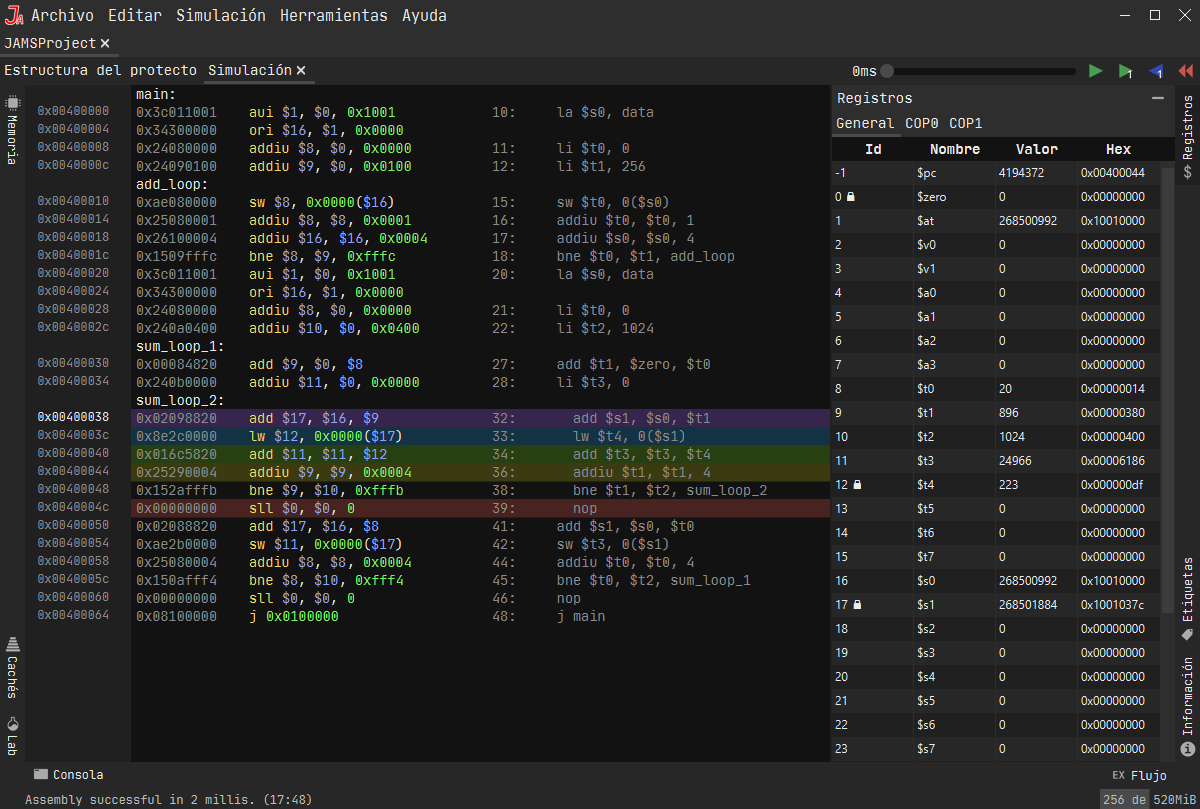
\includegraphics[width=0.8\textwidth]{images/tools/jams-registers}
    \caption{Herramienta de registros}
    \label{fig:jams-registers}
\end{figure}

\noindent En arquitecturas avanzadas, los registros pueden ser
bloqueados por una instrucción.
Cuando un registro está bloqueado, el icono de un candado \faLock \
aparecerá junto con el identificador.

\noindent El usuario puede \textbf{editar los valores de un registro}
haciendo doble clic en la casilla de valor
o valor hexadecimal correspondiente.
Al editar, el usuario puede insertar un valor en decimal,
hexadecimal, octal o binario.
En el caso de los registros del coprocesador 1,
también se pueden insertar valores en coma flotante.
    \chapter{Conclusiones}\label{ch:conclusiones}

Los objetivos de este proyecto estaban asociados a la \textbf{creación
de un nuevo entorno de desarrollo} especializado en lenguajes
ensamblador que pudieran usar tanto desarrolladores avanzados
como alumnos.

\noindent \textit{JAMS} es un entorno de desarrollo moderno,
flexible, modular y fácil de usar, donde el usuario puede
crear aplicaciones de una manera rápida y cómoda,
apoyándose en las diferentes herramientas y
características que la aplicación aporta.

\noindent La aplicación viene empaquetada junto con un
editor, un ensamblador y un simulador para la arquitectura
\textit{MIPS32}, permitiendo personalizar la manera en la
que un proyecto es ejecutado.

\noindent Gracias a la buena elección de tecnologías y
\textit{frameworks}, la experiencia proporcionada por
\textit{JAMS} es altamente personalizable, permitiendo
al usuario usar y crear temas e idiomas.

\noindent Aunque \textit{JAMS} goce de una arquitectura
totalmente modular, aún no tiene la opción de cargar componentes.
Esta característica será implementada en el Trabajo de Fin de
Grado del Grado en Diseño y Desarrollo de Videojuegos.

\section{Líneas futuras}\label{sec:líneas-futuras}

\textit{JAMS} contará con dos actualizaciones importantes en el
futuro cercano.
La primera actualización ya está en desarrollo, mientras que la
segunda actualización requerirá de nueva tecnología que
el equipo de \textit{JAVA} está desarrollando.
\begin{itemize}
    \item \textbf{Soporte para la arquitectura \textit{MIPS32r5}}:
    actualmente, \textit{JAMS} solo soporta proyectos de la revisión 6
    de la arquitectura \textit{MIPS32}.
    Esta revisión cambia la arquitectura en muchos aspectos con respecto
    a la revisión anterior, lo que fuerza a muchas personas a tener
    que migrar gran parte del código de sus proyectos.
    Añadir soporte a la revisión 5 será una tarea relativamente sencilla,
    sabiendo que la revisión 6 añade más características de las que quita.
    \item \textbf{Uso del \textit{Proyecto Valhalla}:} el
    \textit{Proyecto Valhalla}\cite{PROJECT_VALHALLA}, creado en 2014,
    está desarrollando una de las características más esperadas
    por los desarrolladores \textit{JAVA}: \textbf{paso por valor}.
    Esta característica permitirá optimizar de manera considerable
    muchos aspectos de \textit{JAMS}, como son el editor o el simulador.
    Estas nuevas características empezarán su desarrollo cuando esta
    tecnología esté en fase \textit{preview}.
\end{itemize}

\section{Reflexiones finales}\label{sec:reflexiones-finales}

Este ha sido el proyecto más complejo en el que he trabajo:
\textit{JAMS} abarca un montón de conceptos y tecnologías,
desde la simulación de arquitecturas hasta el despliegue de
aplicaciones automatizado, pasando por el renderizado a tiempo
real, la creación de interfaces y la estructuración de un
proyecto grande.

\noindent \textit{JAMS} ha sido una apuesta, un proyecto
que podría haberse derrumbado rápidamente.
Puede considerarse la consolidación de todos los conocimientos
que he adquirido en los últimos años, tanto fuera como dentro
de la universidad.

\noindent Finalmente, agradecer a todas las personas que me han
estado apoyando en este proyecto, a mi familia, amigos y a mis
tutores Óscar y Luis, ya que gracias a ellos este trabajo
ha sido posible.
    \printbibliography[title=Bibliografía]
\end{document}